\documentclass[a4paper,oneside,12pt]{report}
% Package yang diperlukan
\usepackage{graphicx}      % Untuk memasukkan gambar
\usepackage{geometry}      % Untuk mengatur margin halaman
\usepackage{listings}      % Untuk menampilkan blok kode
\usepackage{xcolor}        % Untuk menggunakan warna
\usepackage{float}         % Untuk kontrol penempatan float (seperti gambar)
\usepackage{hyperref}      % Untuk membuat hyperlink (URL, referensi)
\usepackage{natbib}        % Untuk citation dengan \cite{} yang clickable
\usepackage{indentfirst}   % Untuk memberi indentasi pada paragraf pertama setiap seksi
\usepackage{url}           % Untuk format URL
\usepackage{fancyhdr}      % Untuk kustomisasi header dan footer
\usepackage{tocloft}       % Untuk kustomisasi Daftar Isi
\usepackage{bookmark}      % Untuk manajemen bookmark PDF yang lebih baik

%======================================================================
% PENGATURAN GEOMETRI HALAMAN
%======================================================================
% Margin umum untuk isi laporan
\geometry{left=3cm, right=2.5cm, top=2cm, bottom=2.5cm}
\sloppy

%======================================================================
% PENGATURAN WARNA UNTUK BLOK KODE
%======================================================================
\definecolor{codegreen}{rgb}{0,0.6,0}
\definecolor{codegray}{rgb}{0.5,0.5,0.5}
\definecolor{codepurple}{rgb}{0.58,0,0.82}
\definecolor{backcolour}{rgb}{0.95,0.95,0.92}
\definecolor{darkblue}{rgb}{0,0,0.6}

%======================================================================
% PENGATURAN BLOK KODE (LISTINGS)
%======================================================================
% Gaya umum untuk semua blok kode
\lstdefinestyle{commonstyle}{
    backgroundcolor=\color{backcolour}, 
    breakatwhitespace=false, 
    breaklines=true, 
    captionpos=b, 
    keepspaces=true,
    numbers=left, 
    numbersep=5pt, 
    showspaces=false, 
    showstringspaces=false,
    showtabs=false, 
    tabsize=2, 
    frame=single,
    basicstyle=\ttfamily\footnotesize,
    numberstyle=\tiny\color{codegray},
    columns=flexible,
    postbreak=\mbox{\textcolor{red}{$\hookrightarrow$}\space},
    breakindent=0pt,
    breakautoindent=false
}

% Gaya khusus untuk HTML
\lstdefinestyle{htmlstyle}{
    style=commonstyle,
    language=HTML,
    commentstyle=\color{codegreen},
    keywordstyle=\color{codepurple},
    stringstyle=\color{codegreen},
    basicstyle=\ttfamily\scriptsize
}

% Gaya khusus untuk CSS
\lstdefinestyle{cssstyle}{
    style=commonstyle,
    commentstyle=\color{codegreen},
    keywordstyle=\color{darkblue},
    stringstyle=\color{codepurple},
    emph={color, background, font, margin, padding, border, display, position, width, height},
    emphstyle=\color{darkblue},
    basicstyle=\ttfamily\scriptsize
}

% Gaya khusus untuk Python
\lstdefinestyle{pythonstyle}{
    style=commonstyle,
    language=Python,
    commentstyle=\color{codegreen},
    keywordstyle=\color{darkblue},
    stringstyle=\color{codepurple},
    emph={import,from,class,def,for,while,if,else,elif,try,except,finally},
    emphstyle=\color{darkblue}
}

% Gaya khusus untuk SQL
\lstdefinestyle{sqlstyle}{
    style=commonstyle,
    language=SQL,
    commentstyle=\color{codegreen},
    keywordstyle=\color{darkblue},
    stringstyle=\color{codepurple},
    emph={SELECT,FROM,WHERE,INSERT,UPDATE,DELETE,CREATE,DROP},
    emphstyle=\color{darkblue}
}

% Gaya khusus untuk JavaScript
\lstdefinestyle{javascriptstyle}{
    style=commonstyle,
    language=JavaScript,
    commentstyle=\color{codegreen},
    keywordstyle=\color{darkblue},
    stringstyle=\color{codepurple},
    emph={function,var,let,const,return,if,for,while,do,else,switch,case},
    emphstyle=\color{darkblue}
}

% Gaya khusus untuk Java
\lstdefinestyle{javastyle}{
    style=commonstyle,
    language=Java,
    commentstyle=\color{codegreen},
    keywordstyle=\color{darkblue}\bfseries,
    stringstyle=\color{codepurple},
    emph={@Test,@Mock,@InjectMocks,@ExtendWith},
    emphstyle=\color{codepurple}
}

%======================================================================
% PENGATURAN LAIN-LAIN
%======================================================================

% Mengganti nama default "Figure" menjadi "Gambar"
\renewcommand{\figurename}{Gambar}
\renewcommand{\thefigure}{\arabic{figure}}

% Pengaturan Hyperlink
\hypersetup{
    colorlinks=true, 
    linkcolor=black, 
    filecolor=black, 
    urlcolor=black,
    citecolor=blue,
    pdftitle={Laporan Praktikum}, 
    pdfpagemode=FullScreen, 
    breaklinks=true
}

% Pengaturan citation style
\bibliographystyle{plain}

% Pengaturan Header & Footer (nomor halaman di tengah bawah)
\pagestyle{fancy}
\fancyhf{}
\fancyfoot[C]{\thepage}
\renewcommand{\headrulewidth}{0pt}

\fancypagestyle{plain}{
    \fancyhf{}
    \fancyfoot[C]{\thepage}
    \renewcommand{\headrulewidth}{0pt}
}

%======================================================================
% PENGATURAN STRUKTUR BAB DAN DAFTAR ISI
%======================================================================
\renewcommand{\contentsname}{Daftar Isi}
\renewcommand{\bibname}{Daftar Pustaka}

% Menghilangkan nomor bab tetapi mempertahankan penomoran seksi
\renewcommand{\thechapter}{}
\renewcommand{\chaptername}{}

% Format penomoran seksi menjadi [nomor bab].[nomor seksi]
\renewcommand{\thesection}{\arabic{chapter}.\arabic{section}}
\renewcommand{\thesubsection}{\thesection.\arabic{subsection}}

\setcounter{secnumdepth}{3}
\setcounter{tocdepth}{2}

% Format Daftar Isi (TOC)
\renewcommand{\cftchapdotsep}{\cftdotsep}
\renewcommand{\cftchapleader}{\cftdotfill{\cftchapdotsep}}
\setlength{\cftchapindent}{0em}
\setlength{\cftsecindent}{2em}
\setlength{\cftsubsecindent}{4em}
\setlength{\cftchapnumwidth}{0em}
\setlength{\cftsecnumwidth}{2.5em}
\setlength{\cftsubsecnumwidth}{3.2em}
\renewcommand{\cftchappresnum}{}
\renewcommand{\cftchapaftersnum}{}

% Perintah kustom untuk membuat judul bab di TOC menjadi tebal
\newcommand{\tocboldsection}[1]{%
  \protect\renewcommand{\protect\cftchapfont}{\protect\bfseries}%
  #1%
  \protect\renewcommand{\protect\cftchapfont}{}%
}

%======================================================================
% AWAL DOKUMEN
%======================================================================
\begin{document}

% Halaman Judul
\newgeometry{left=3cm, right=2.5cm, top=2.5cm, bottom=3cm}
\begin{titlepage}
\begin{center}
\vspace*{0.5cm}
{\large \textbf{\MakeUppercase{Laporan Praktikum}}} \\[0.4cm]
{\large \textbf{\MakeUppercase{PRAKTIKUM PENGUJIAN PERANGKAT LUNAK}}} \\[0.4cm]
{\large \textbf{\MakeUppercase{Pertemuan 5}}} \\[0.4cm]
{\large \textbf{\MakeUppercase{Test Document}}} \\[1.5cm]


\includegraphics[height=7cm]{lambang ugm.png} \\[1cm]

{\normalsize \textbf{Disusun oleh:}} \\[0.4cm]
\begin{tabular}{@{}l l @{}}
  \textbf{Nama}           & : Januarsyah Akbar \\
  \textbf{NIM}            & : 24/535846/SV/24314 \\
  \textbf{Kelas}          & : PL4B2 \\
    \textbf{Dosen Pengampu} & : Divi Galih Prasetyo Putri, S.Kom., M.Kom., Ph.D.
\end{tabular} \\[1.2cm]

{\normalsize \textbf{PROGRAM STUDI D-IV}} \\[0.2cm]
{\normalsize \textbf{TEKNOLOGI REKAYASA PERANGKAT LUNAK}} \\[0.2cm]
{\normalsize \textbf{DEPARTEMEN TEKNIK ELEKTRO DAN INFORMATIKA}} \\[0.2cm]
{\normalsize \textbf{SEKOLAH VOKASI}} \\[0.2cm]
{\normalsize \textbf{UNIVERSITAS GADJAH MADA}} \\[0.2cm]
{\normalsize \textbf{YOGYAKARTA}} \\[0.2cm]
{\normalsize \textbf{\today}} \\[1.2cm]
\end{center}
\end{titlepage}
\restoregeometry

\thispagestyle{empty}
\clearpage
\stepcounter{page}
\thispagestyle{empty}

% --- Daftar Isi ---
\addcontentsline{toc}{chapter}{Daftar Isi}
\tableofcontents
\clearpage

% Mengatur penomoran halaman menjadi arab dan mulai dari 3
\pagenumbering{arabic}
\setcounter{page}{3}

%======================================================================
\chapter[Tujuan Praktikum]{Tujuan Praktikum}
%======================================================================
\begin{enumerate}
    \item Mahasiswa mampu memahami definisi, fungsi, dan cara pembuatan skenario pengujian serta pelaporan bug.
    \item Mahasiswa mampu membuat skenario pengujian serta pelaporan bug.
\end{enumerate}
\clearpage

%======================================================================
\chapter[\tocboldsection{Hasil dan Pembahasan}]{Hasil dan Pembahasan}
%======================================================================

%----------------------------------------------------------------------
\section{Tugas}
%----------------------------------------------------------------------

Berikut adalah penjelasan dan langkah-langkah praktikum terkait pembuatan \textit{Test Document} menggunakan Qase sesuai dengan urutan tangkapan layar yang telah dilakukan:

\subsection{Langkah 1: Membuat Project Baru}
Langkah pertama yang dilakukan adalah membuat sebuah \textit{project} baru pada \textit{platform} manajemen pengujian. \textit{project} ini akan menjadi tempat pengelolaan seluruh aktivitas \textit{testing} pada suatu perangkat lunak.
\begin{figure}[H]
    \centering
    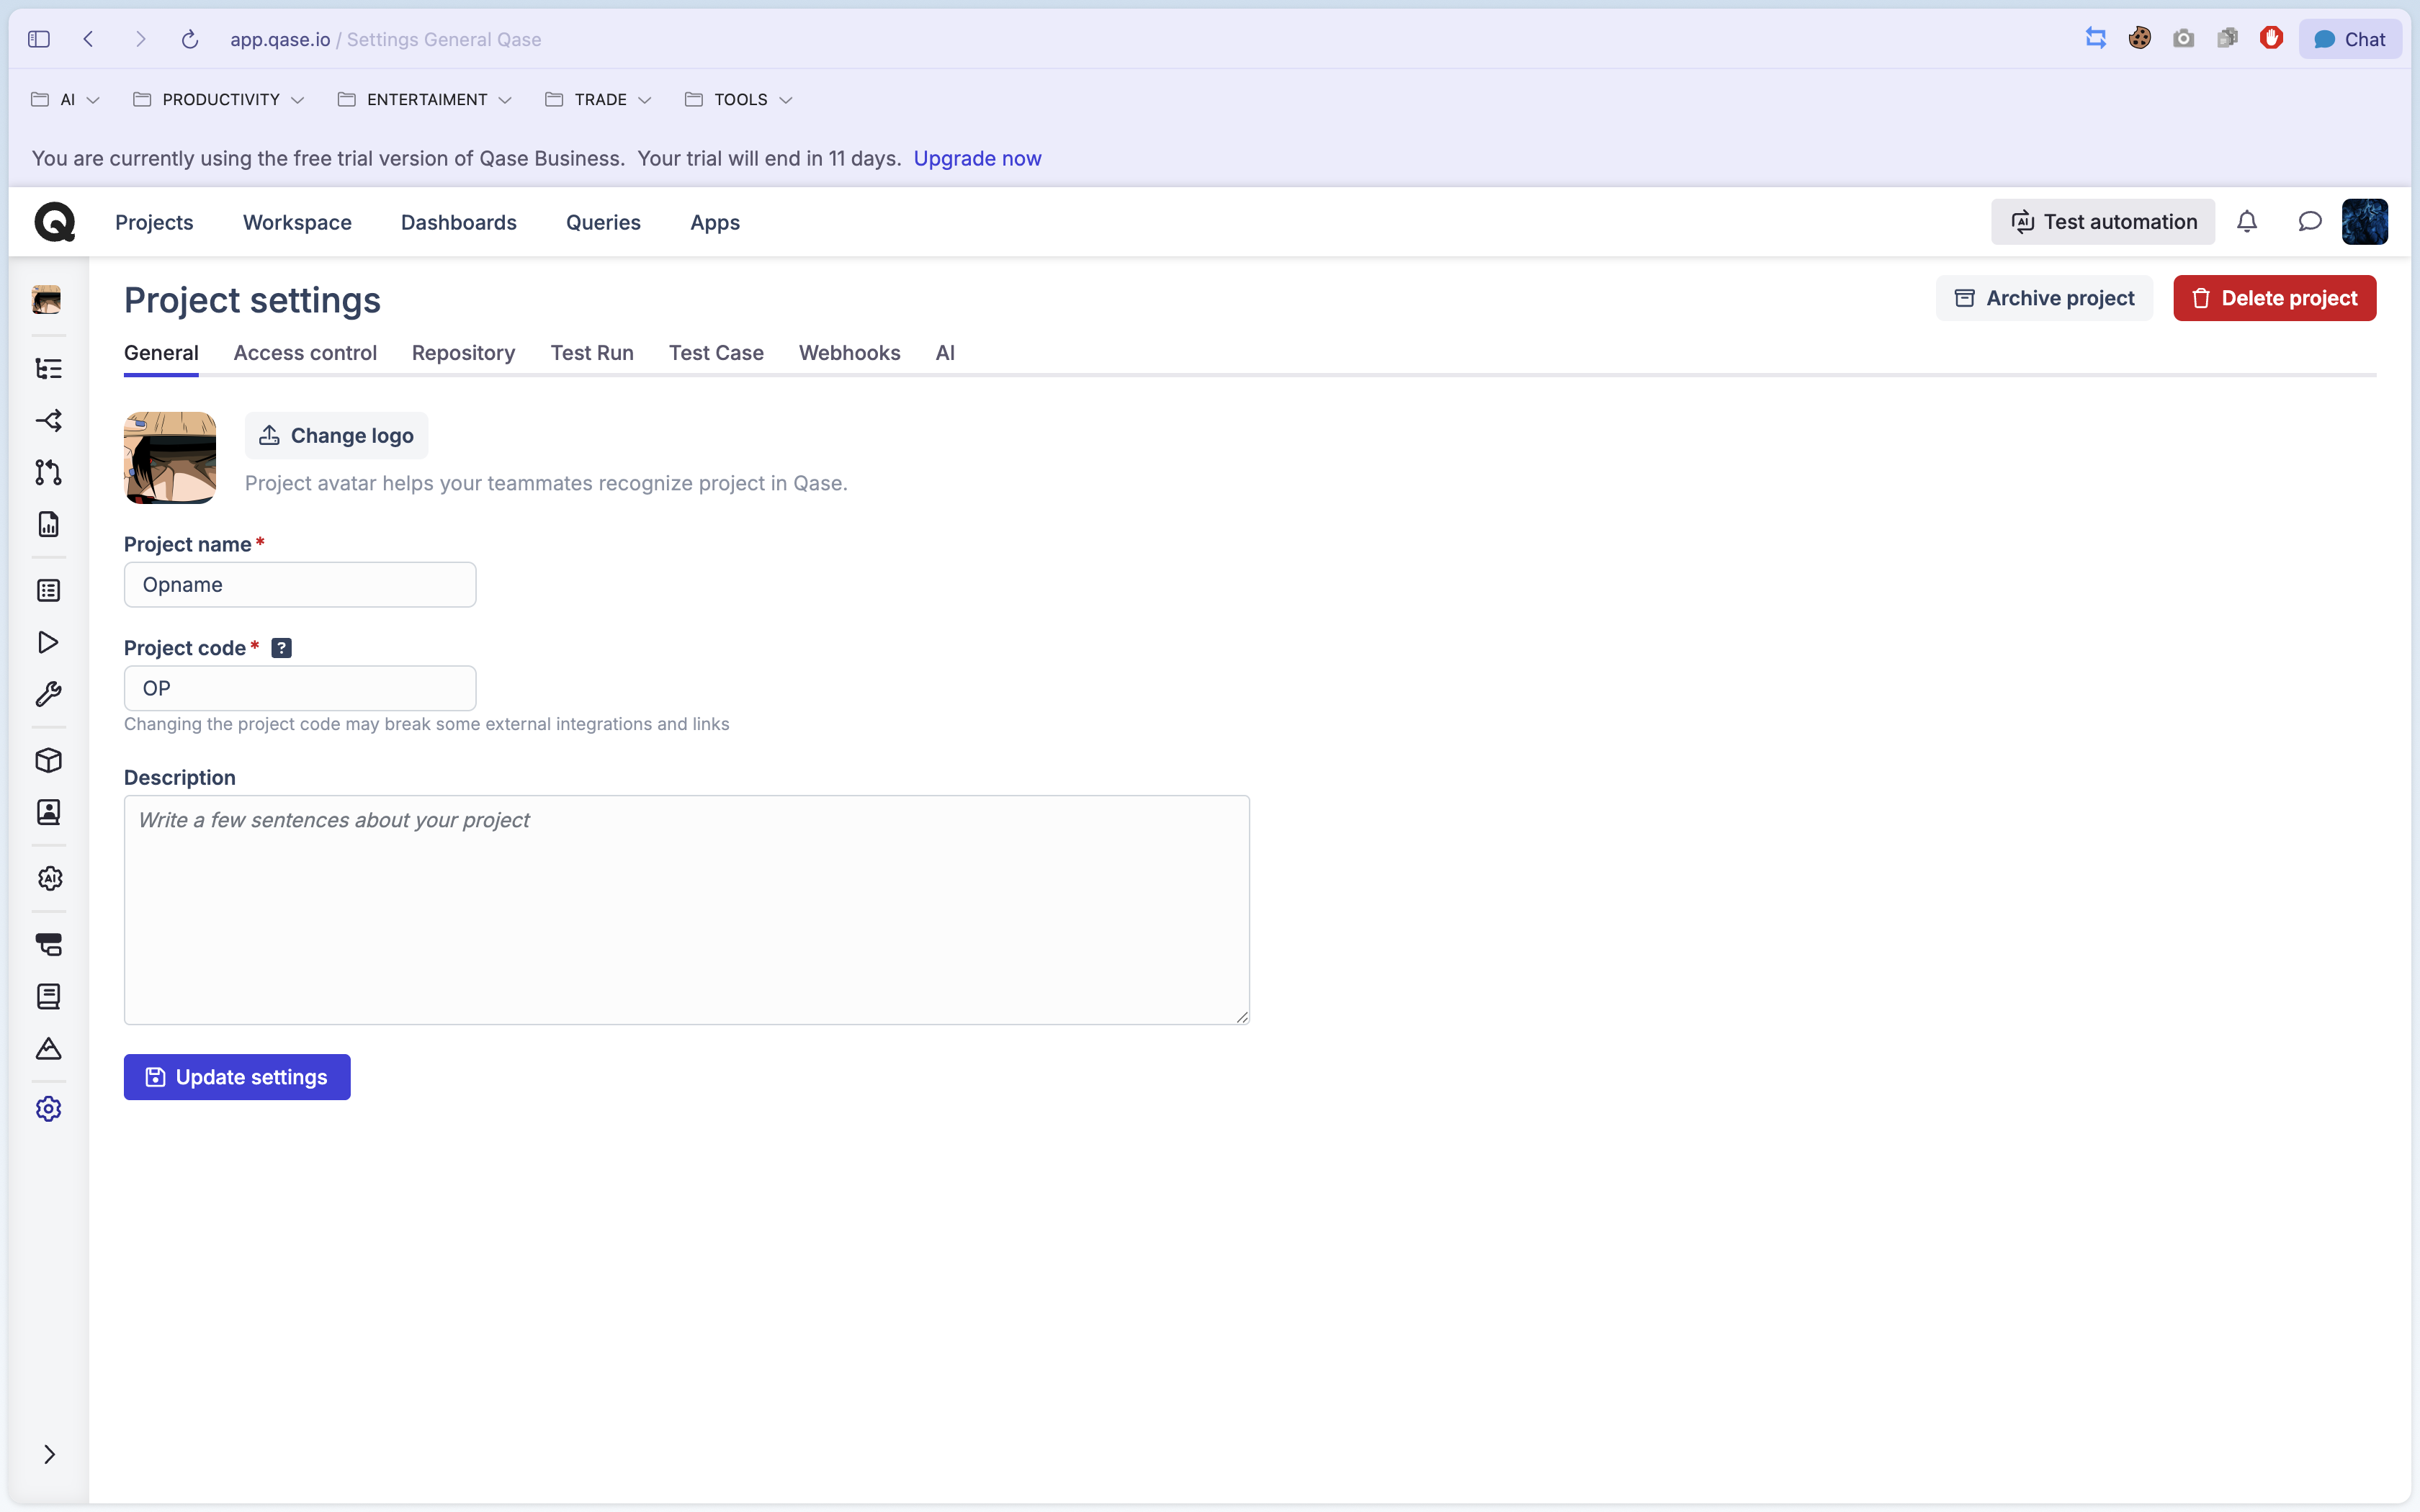
\includegraphics[width=\textwidth]{screenshot step/01-new project.png}
    \caption{Membuat Project Baru}
\end{figure}

\subsection{Langkah 2: Membuat Test Suite}
Selanjutnya, kita membuat \textit{Test Suite} untuk mengelompokkan berbagai \textit{Test Case} yang terkait, misalnya mengatur pengujian berdasarkan modul tertentu yang ada di aplikasi.
\begin{figure}[H]
    \centering
    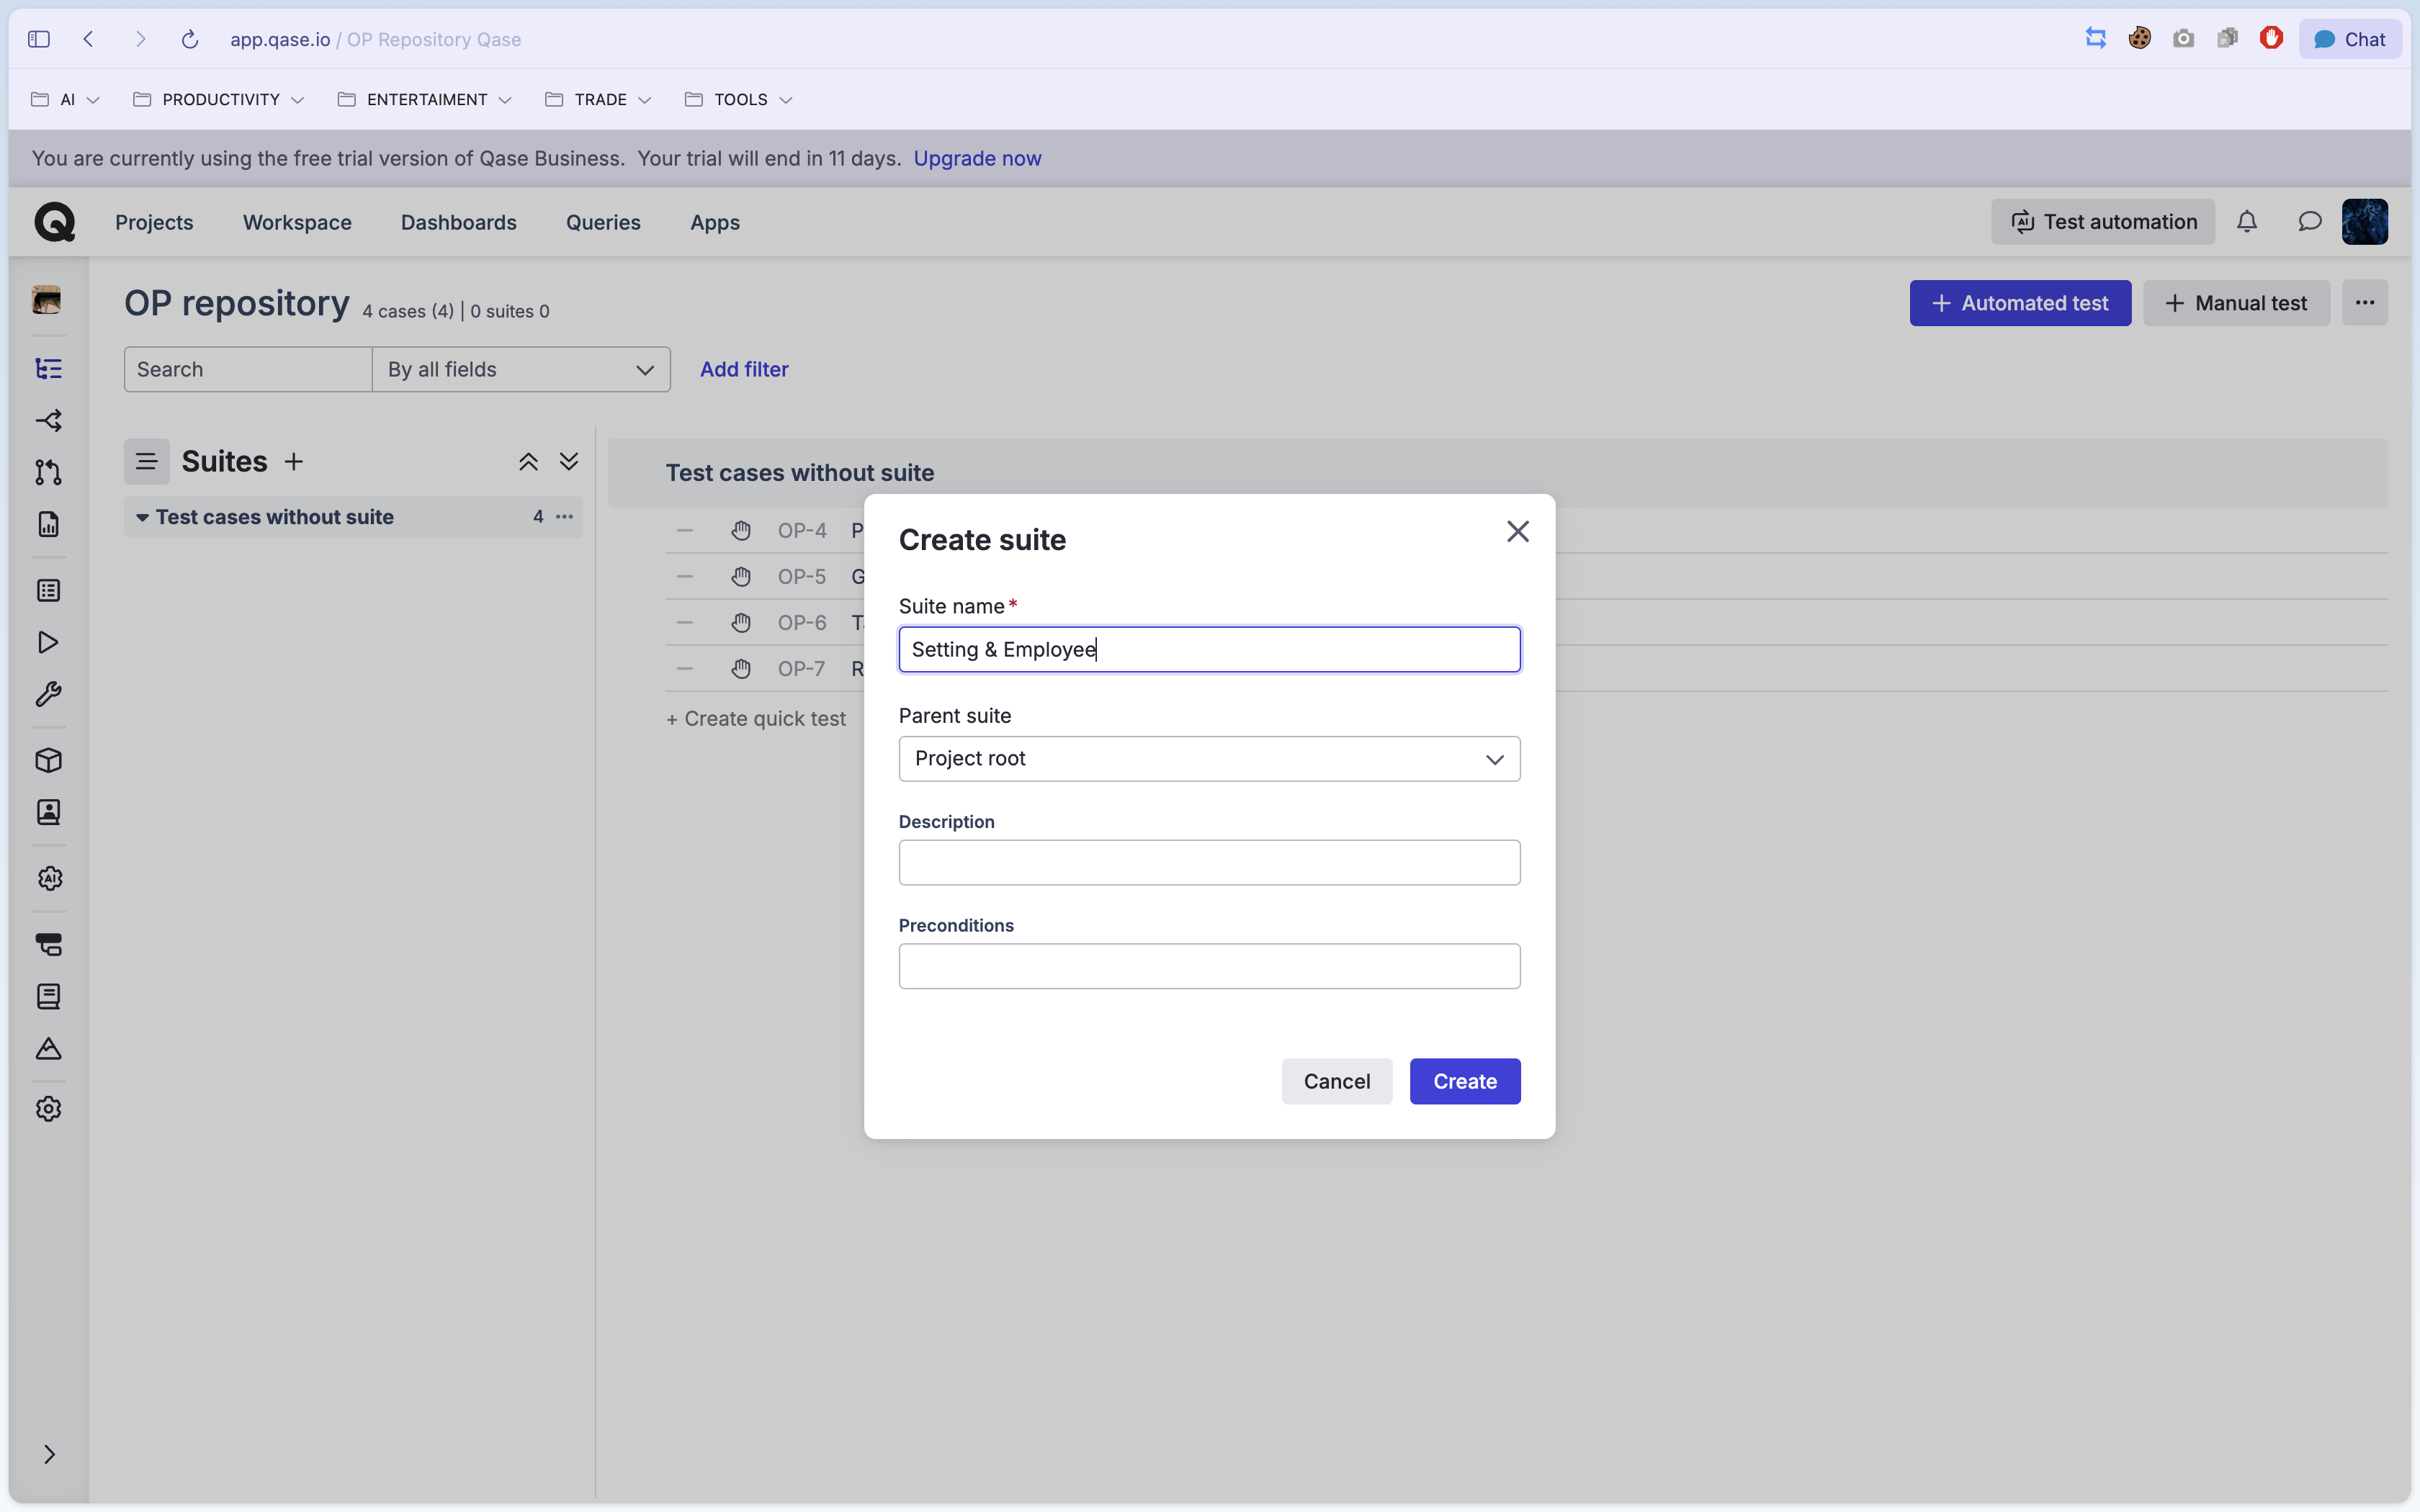
\includegraphics[width=\textwidth]{screenshot step/02-create suite.png}
    \caption{Membuat Test Suite}
\end{figure}

\subsection{Langkah 3: Membuat Test Case}
Kemudian, kita merancang spesifikasi dan langkah-langkah pengujian di dalam \textit{Test Case}, mencakup aksi yang harus dilakukan dan \textit{expected result}, untuk memastikan apakah sebuah fitur berfungsi sesuai kebutuhan.
\begin{figure}[H]
    \centering
    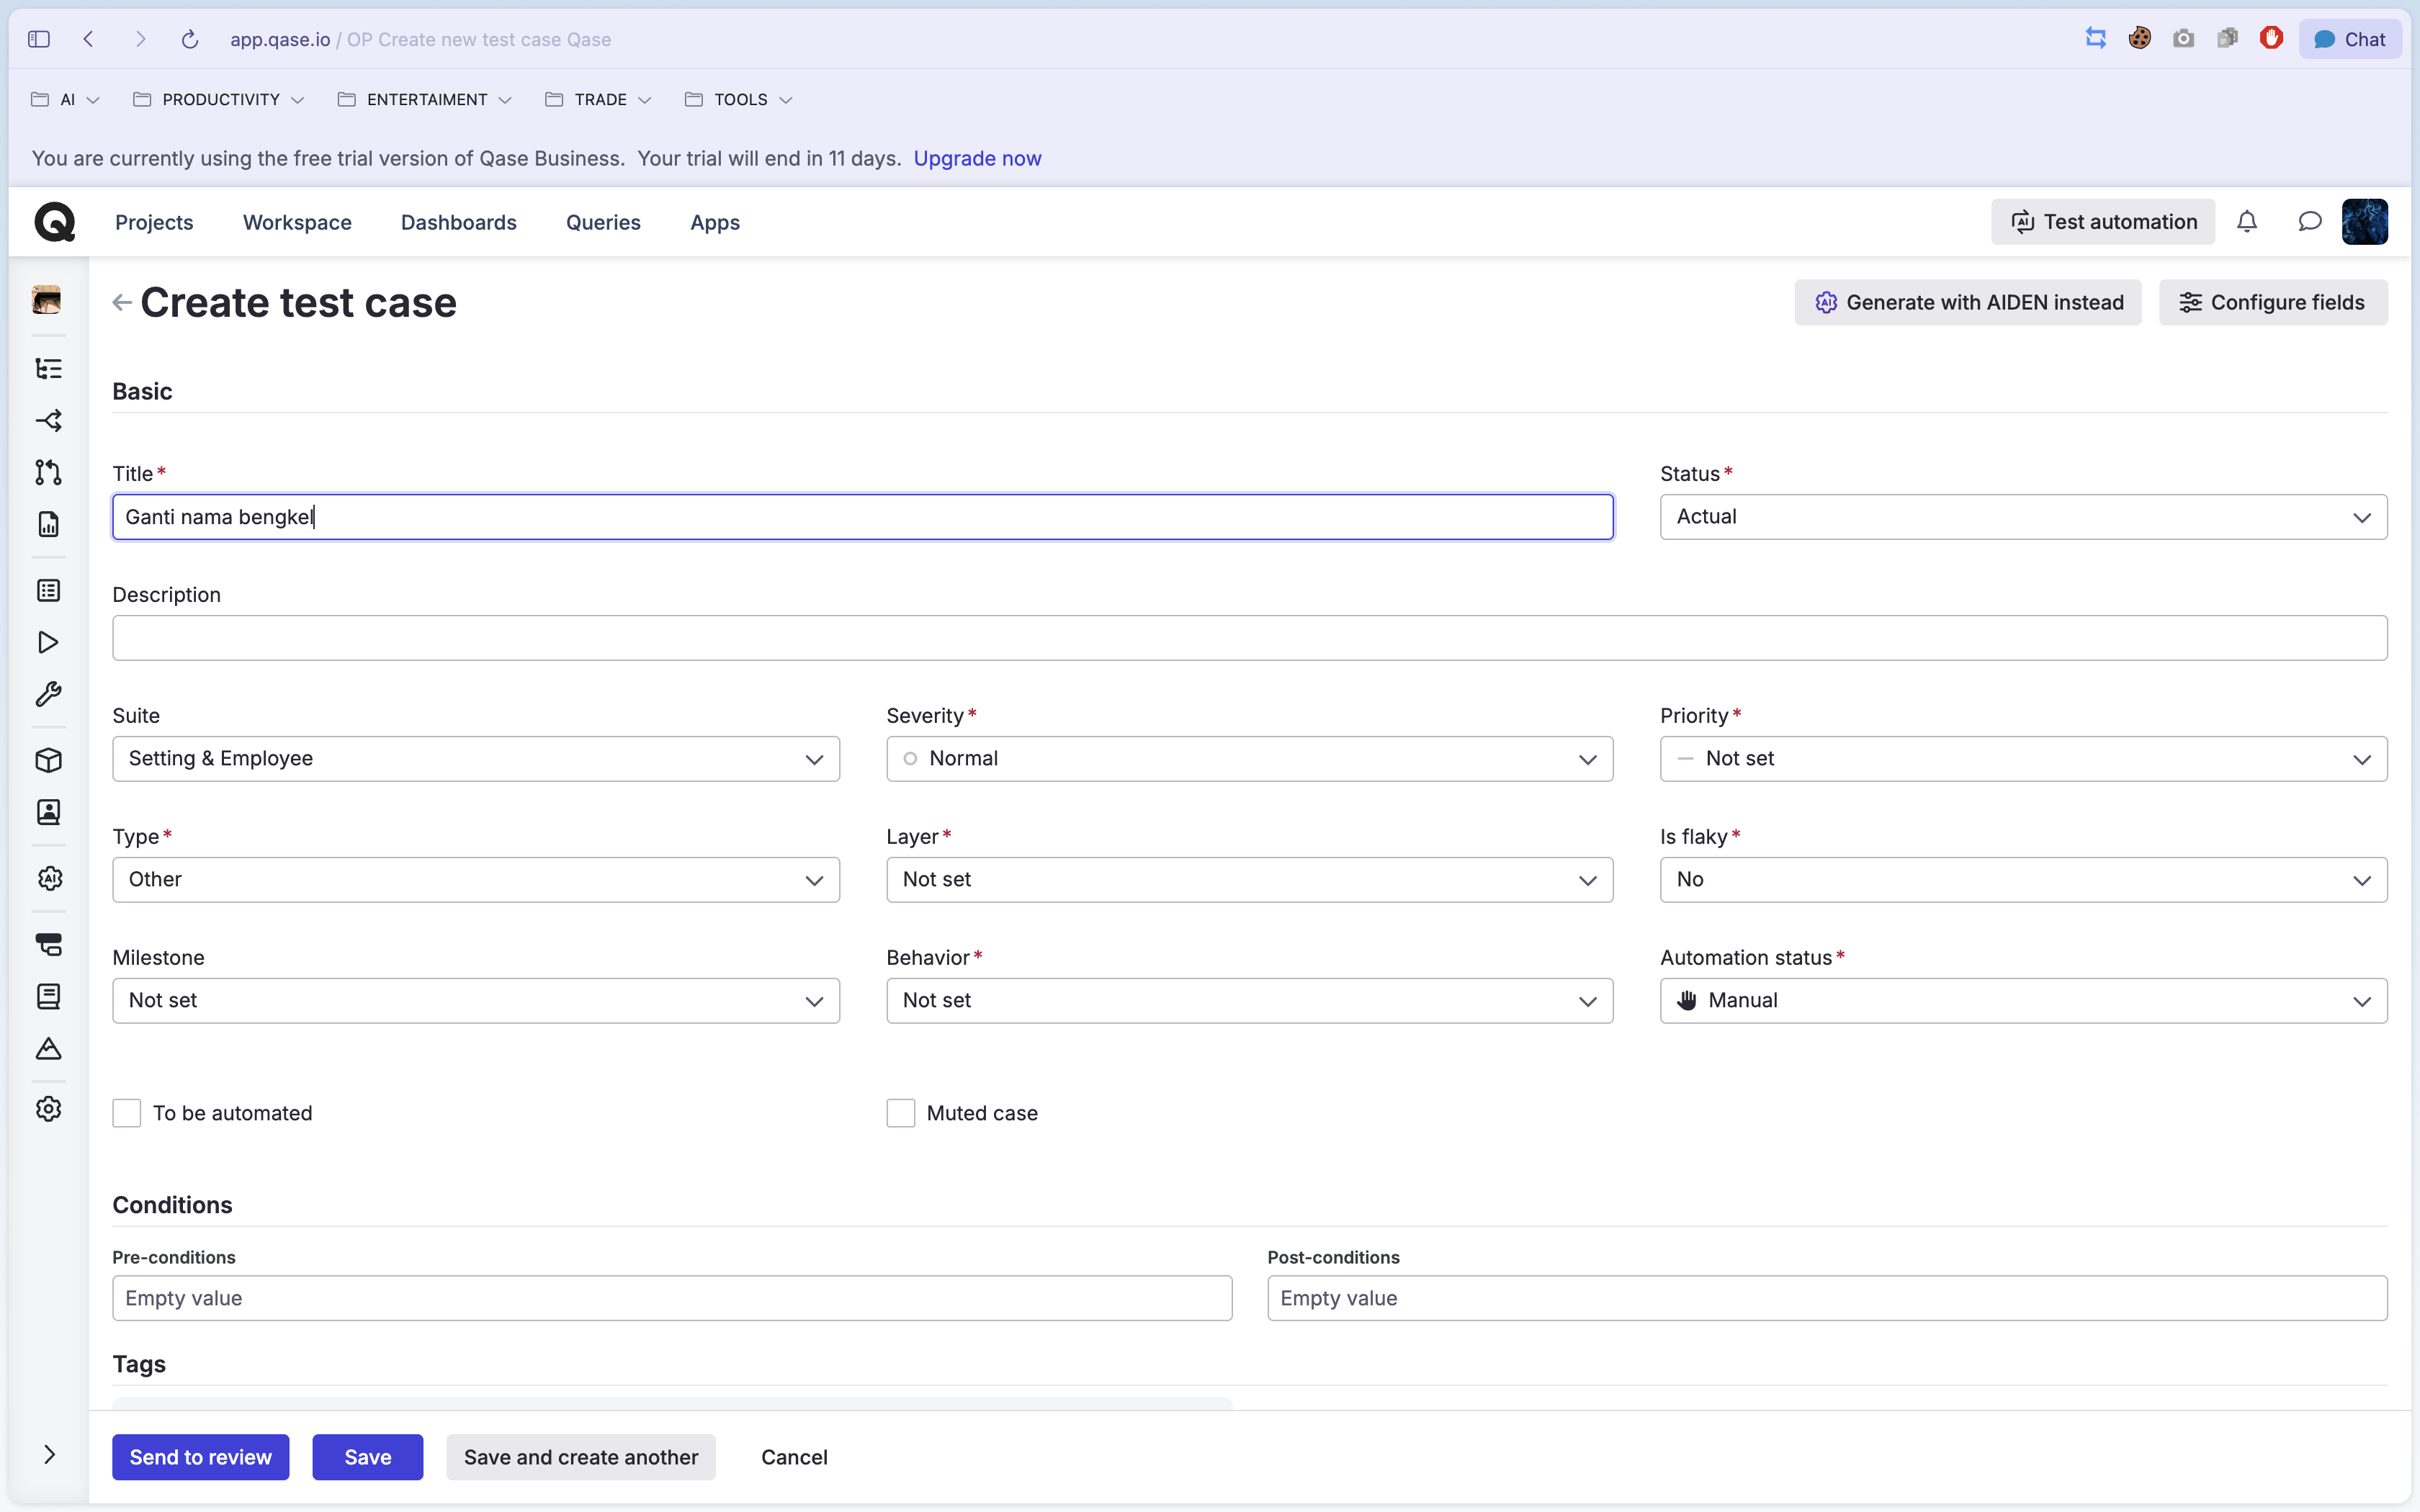
\includegraphics[width=\textwidth]{screenshot step/03-create test case.png}
    \caption{Membuat Test Case}
\end{figure}

\subsection{Langkah 4: Menampilkan Seluruh Test Case}
Setelah beberapa \textit{Test Case} selesai didaftarkan, kita dapat meninjau seluruh daftar \textit{Test Case} yang tersedia pada \textit{Test Suite} secara keseluruhan.
\begin{figure}[H]
    \centering
    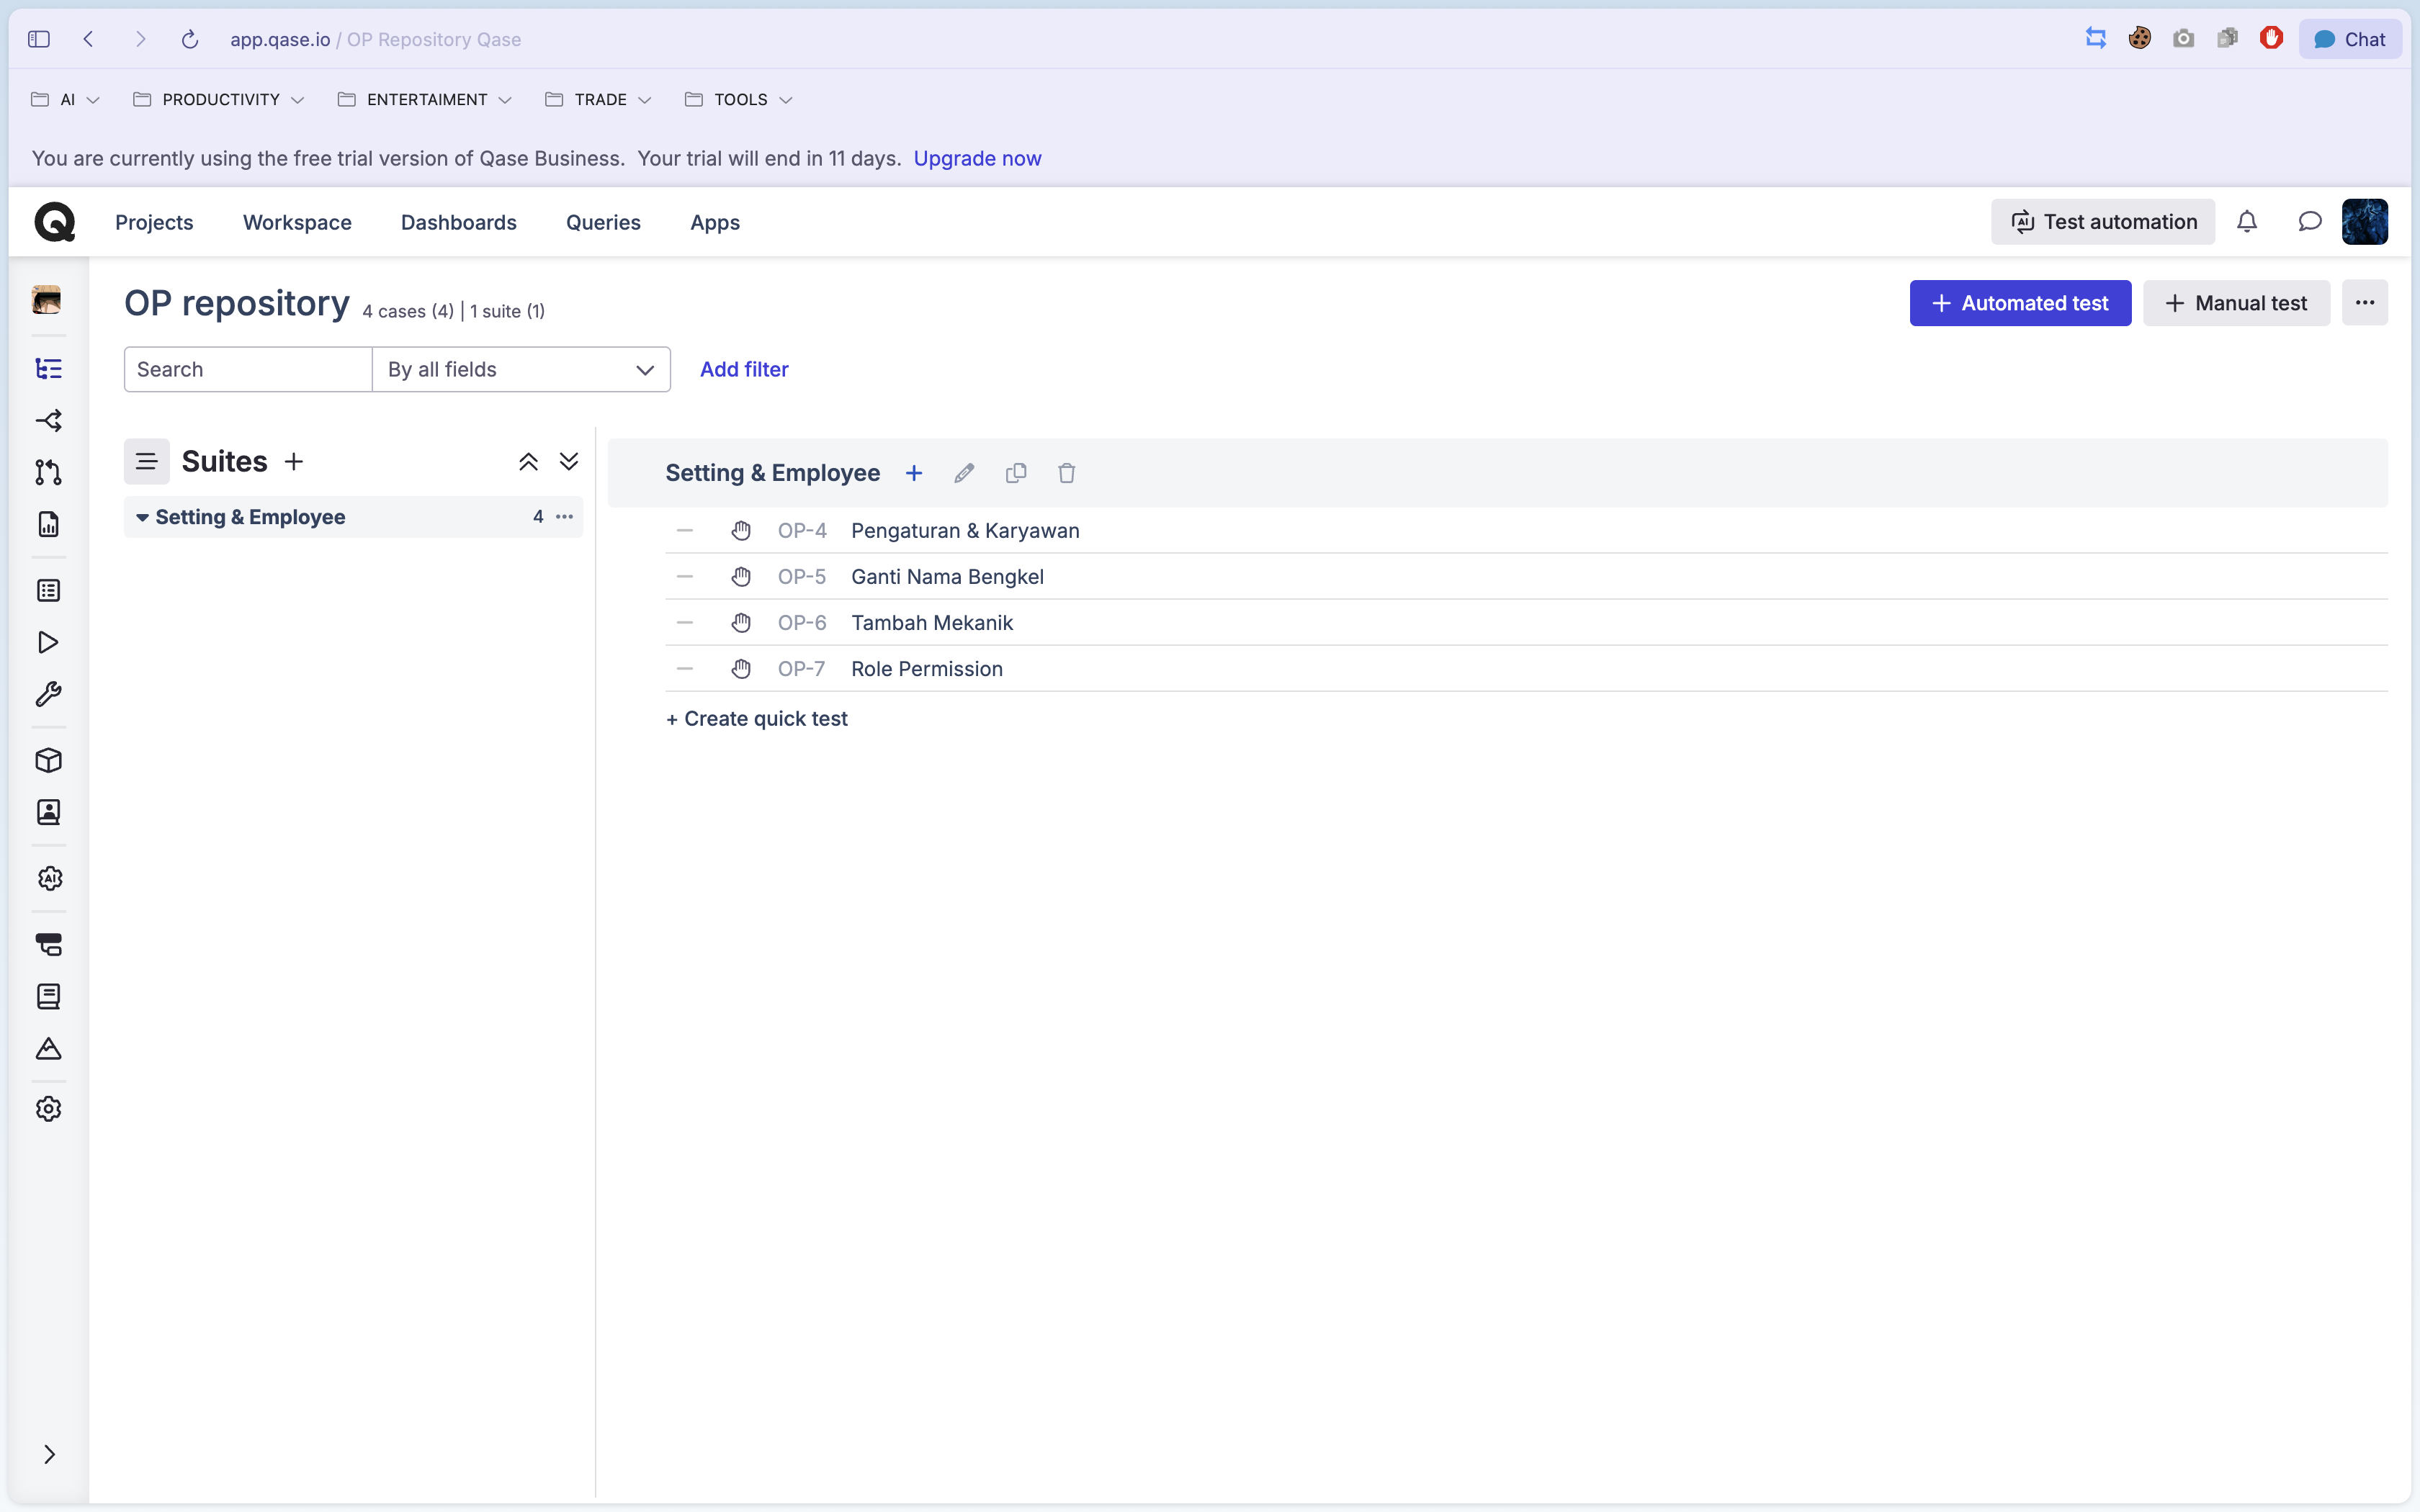
\includegraphics[width=\textwidth]{screenshot step/04-all test case.png}
    \caption{Menampilkan Seluruh Test Case}
\end{figure}

\subsection{Langkah 5: Mengubah/Mengedit Test Case}
Apabila diperlukan penyempurnaan, seperti modifikasi kondisi yang diuji atau mengubah langkahnya, detail pada sebuah \textit{Test Case} tersebut dapat langsung diedit atau diperbarui.
\begin{figure}[H]
    \centering
    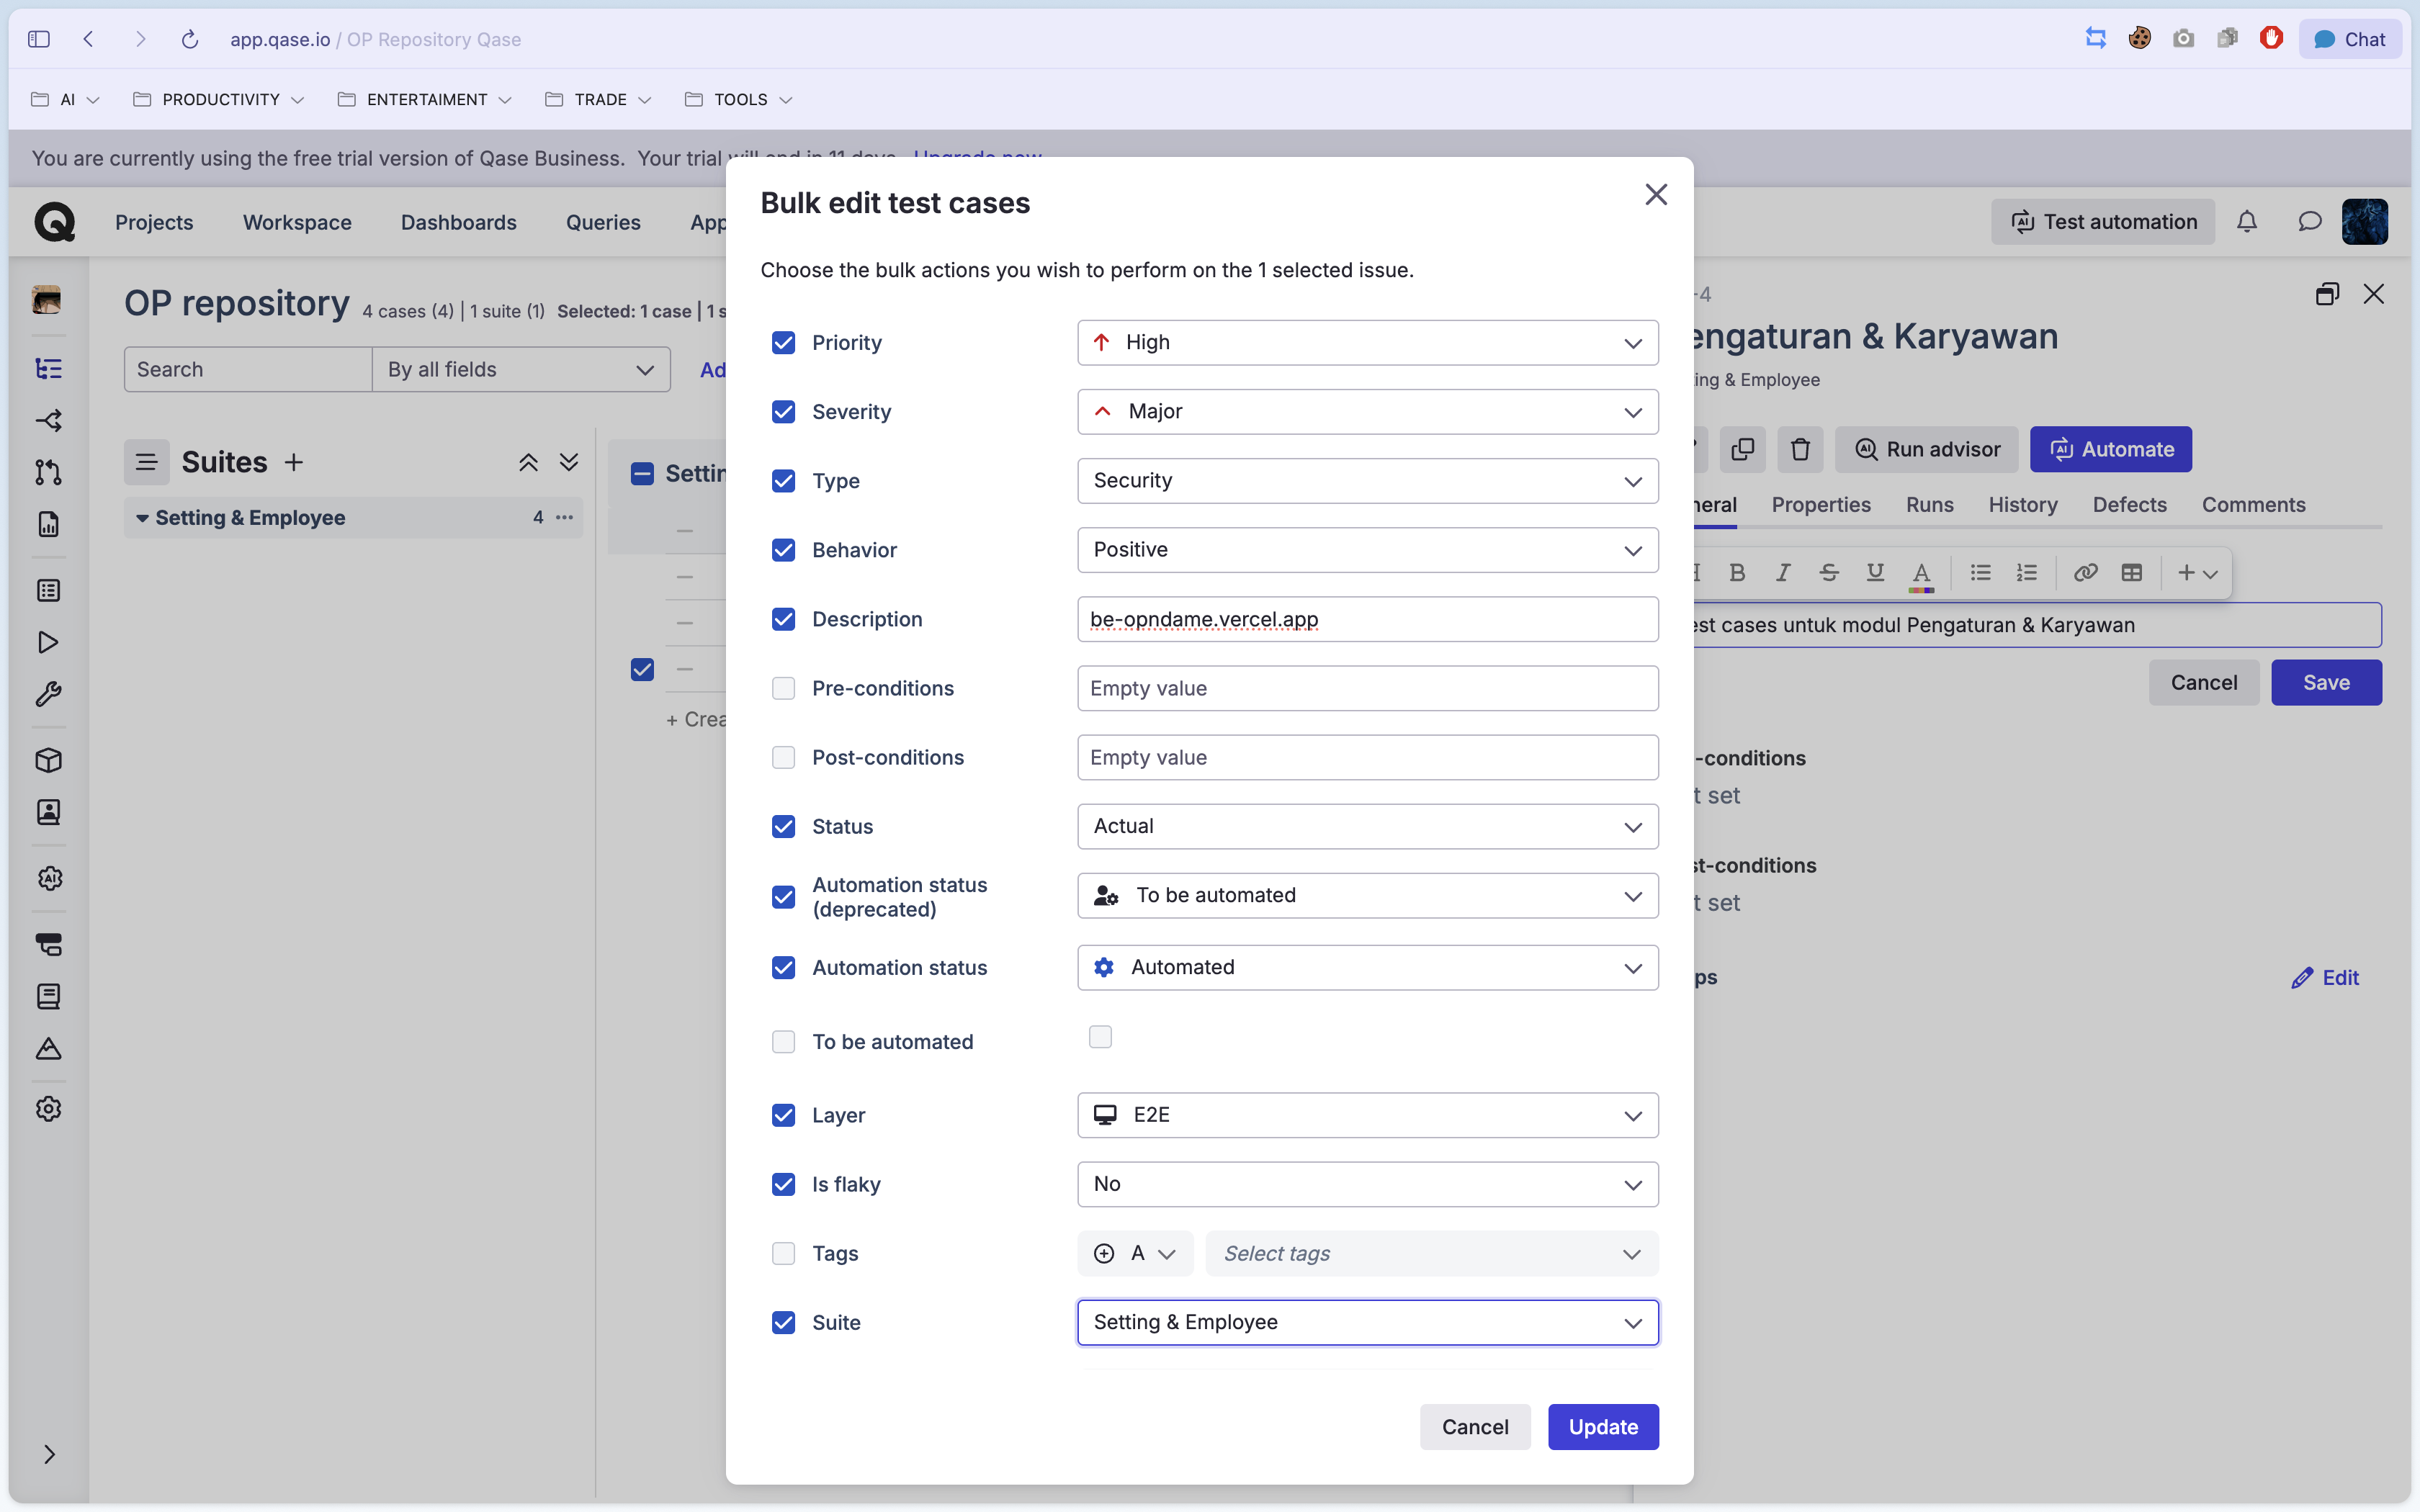
\includegraphics[width=\textwidth]{screenshot step/05-edit test case.png}
    \caption{Mengedit Test Case}
\end{figure}

\subsection{Langkah 6: Membuat Shared Step}
Untuk efisiensi pembuatan \textit{test case}, suatu tahapan yang berulang dan identik diberbagai \textit{test case} dapat didaftarkan sebagai \textit{Shared Step}.
\begin{figure}[H]
    \centering
    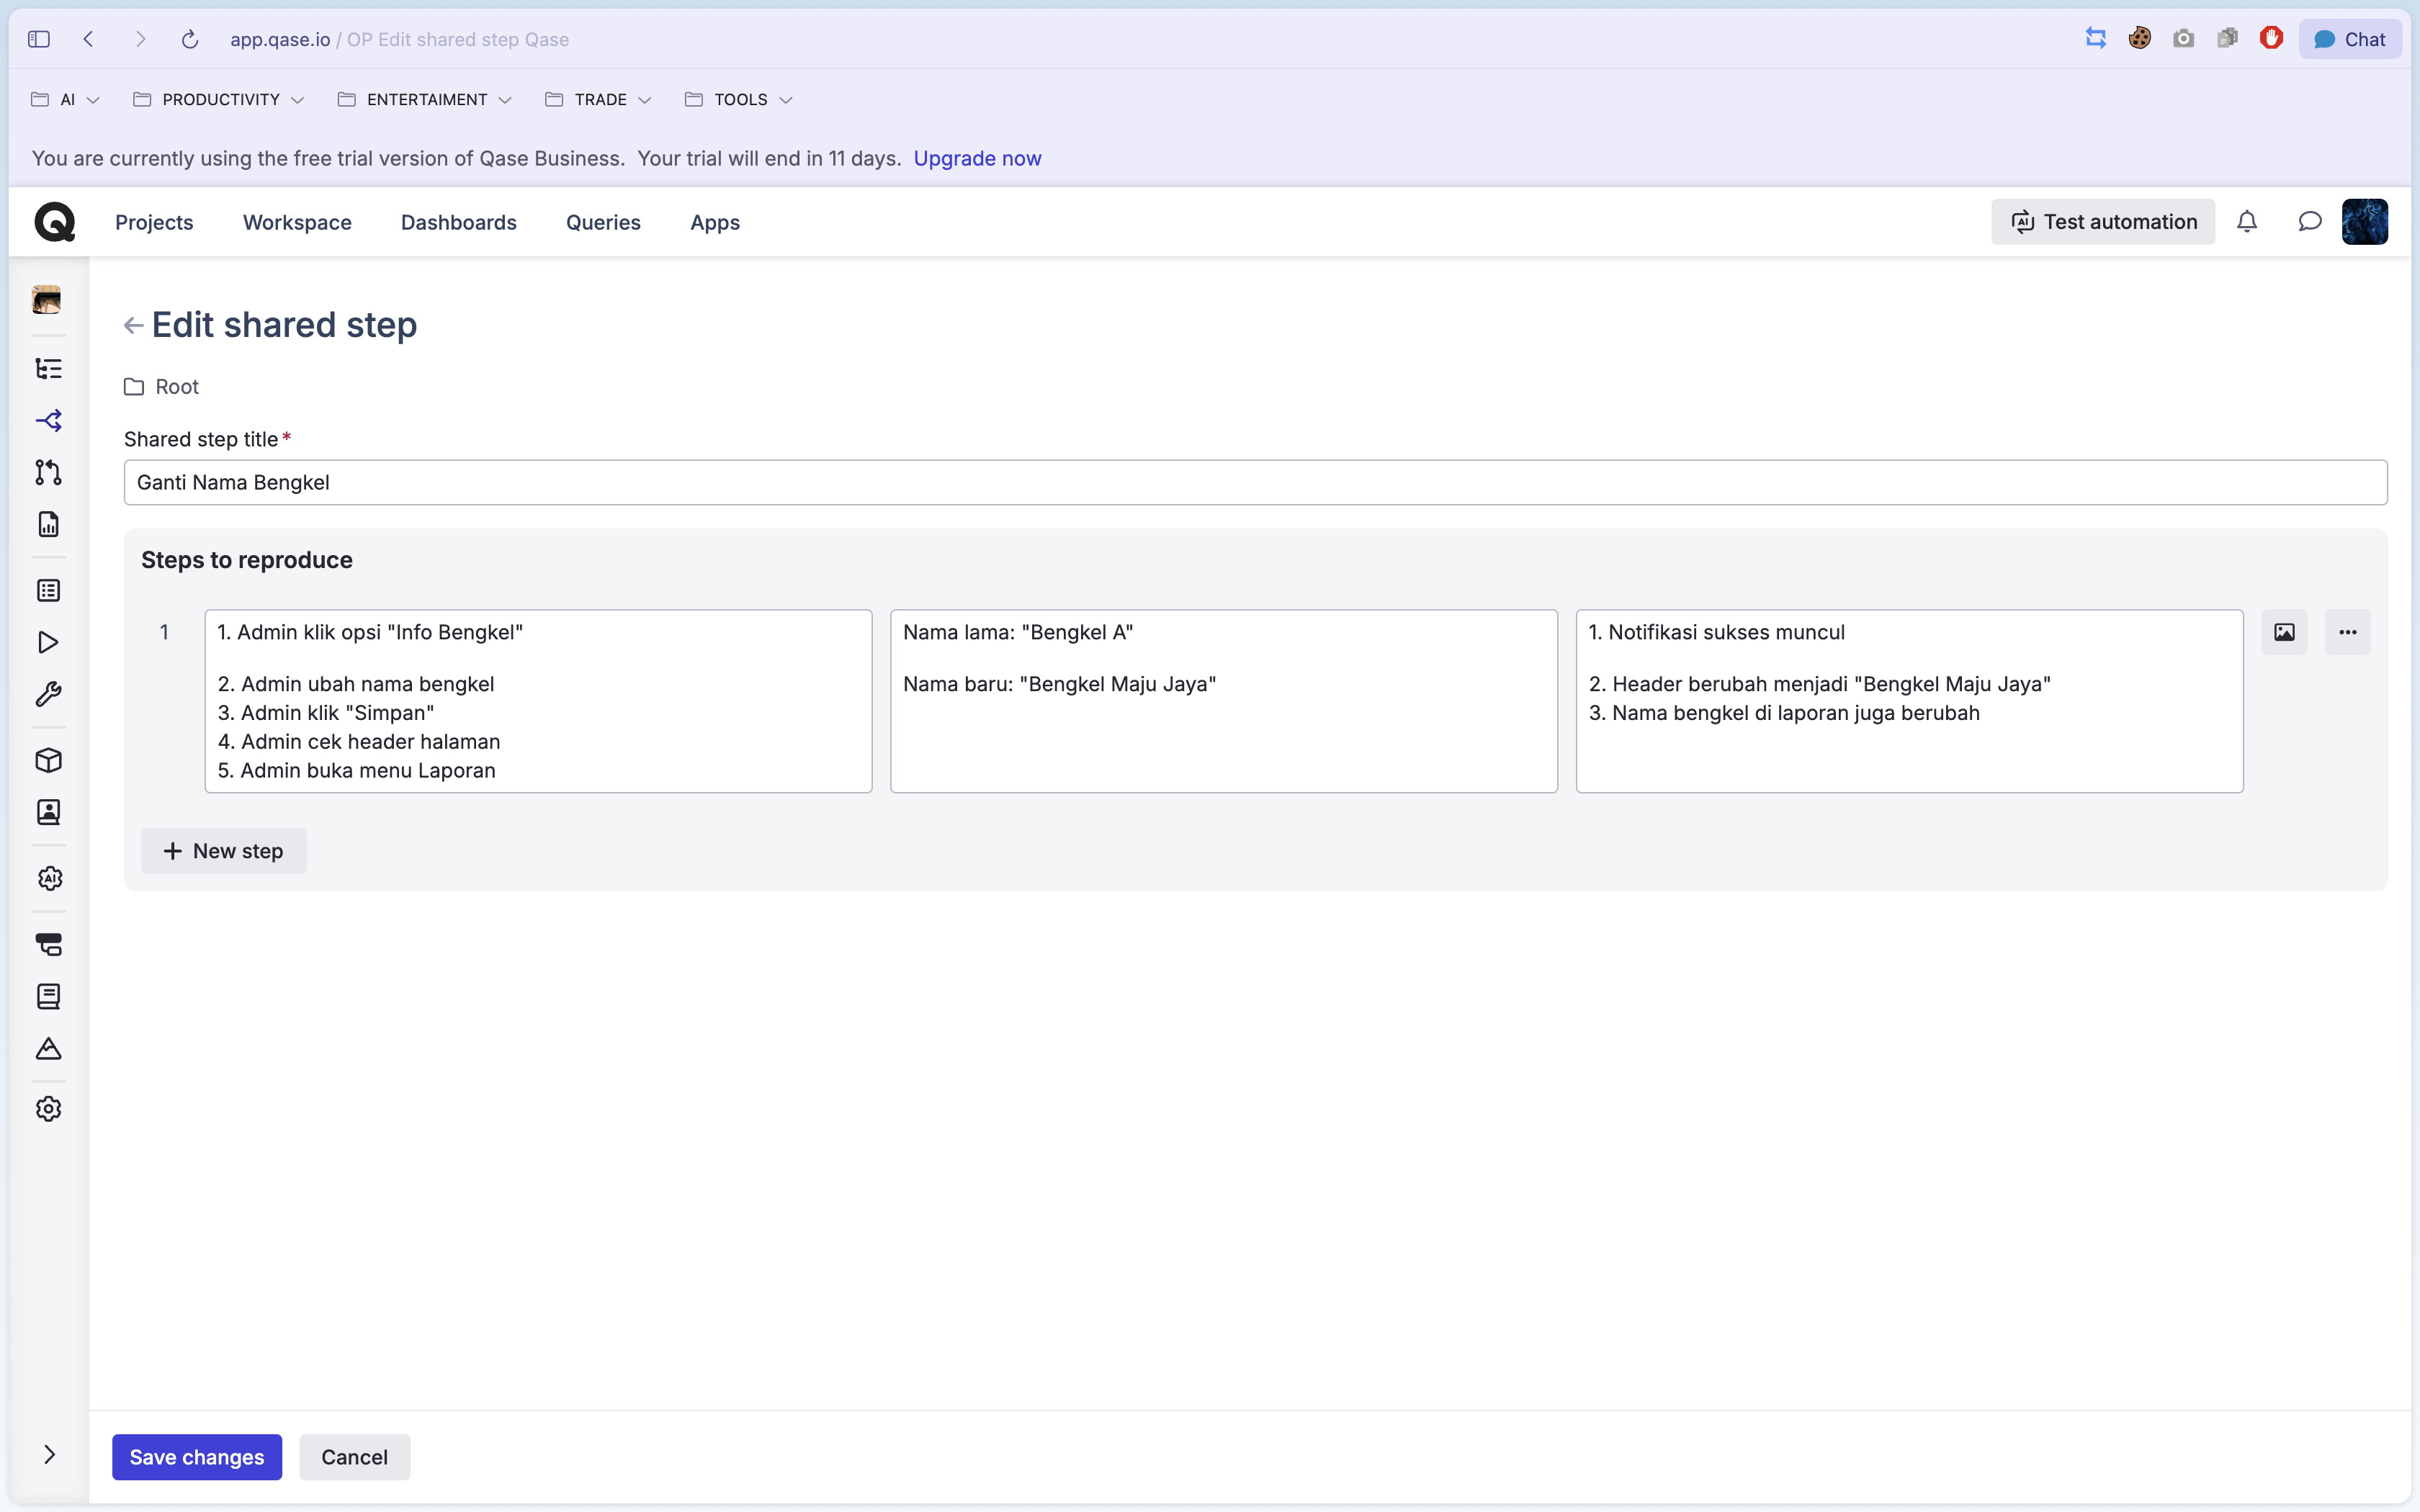
\includegraphics[width=\textwidth]{screenshot step/06-create shared step.png}
    \caption{Membuat Shared Step}
\end{figure}

\subsection{Langkah 7: Konfigurasi Shared Step ke Test Case}
Setelah \textit{Shared Step} berhasil dibuat, kita memanggil \textit{Shared Step} tersebut lalu menyisipkannya pada langkah-langkah di \textit{Test Case} terkait sehingga meminimalisir penulisan berulang.
\begin{figure}[H]
    \centering
    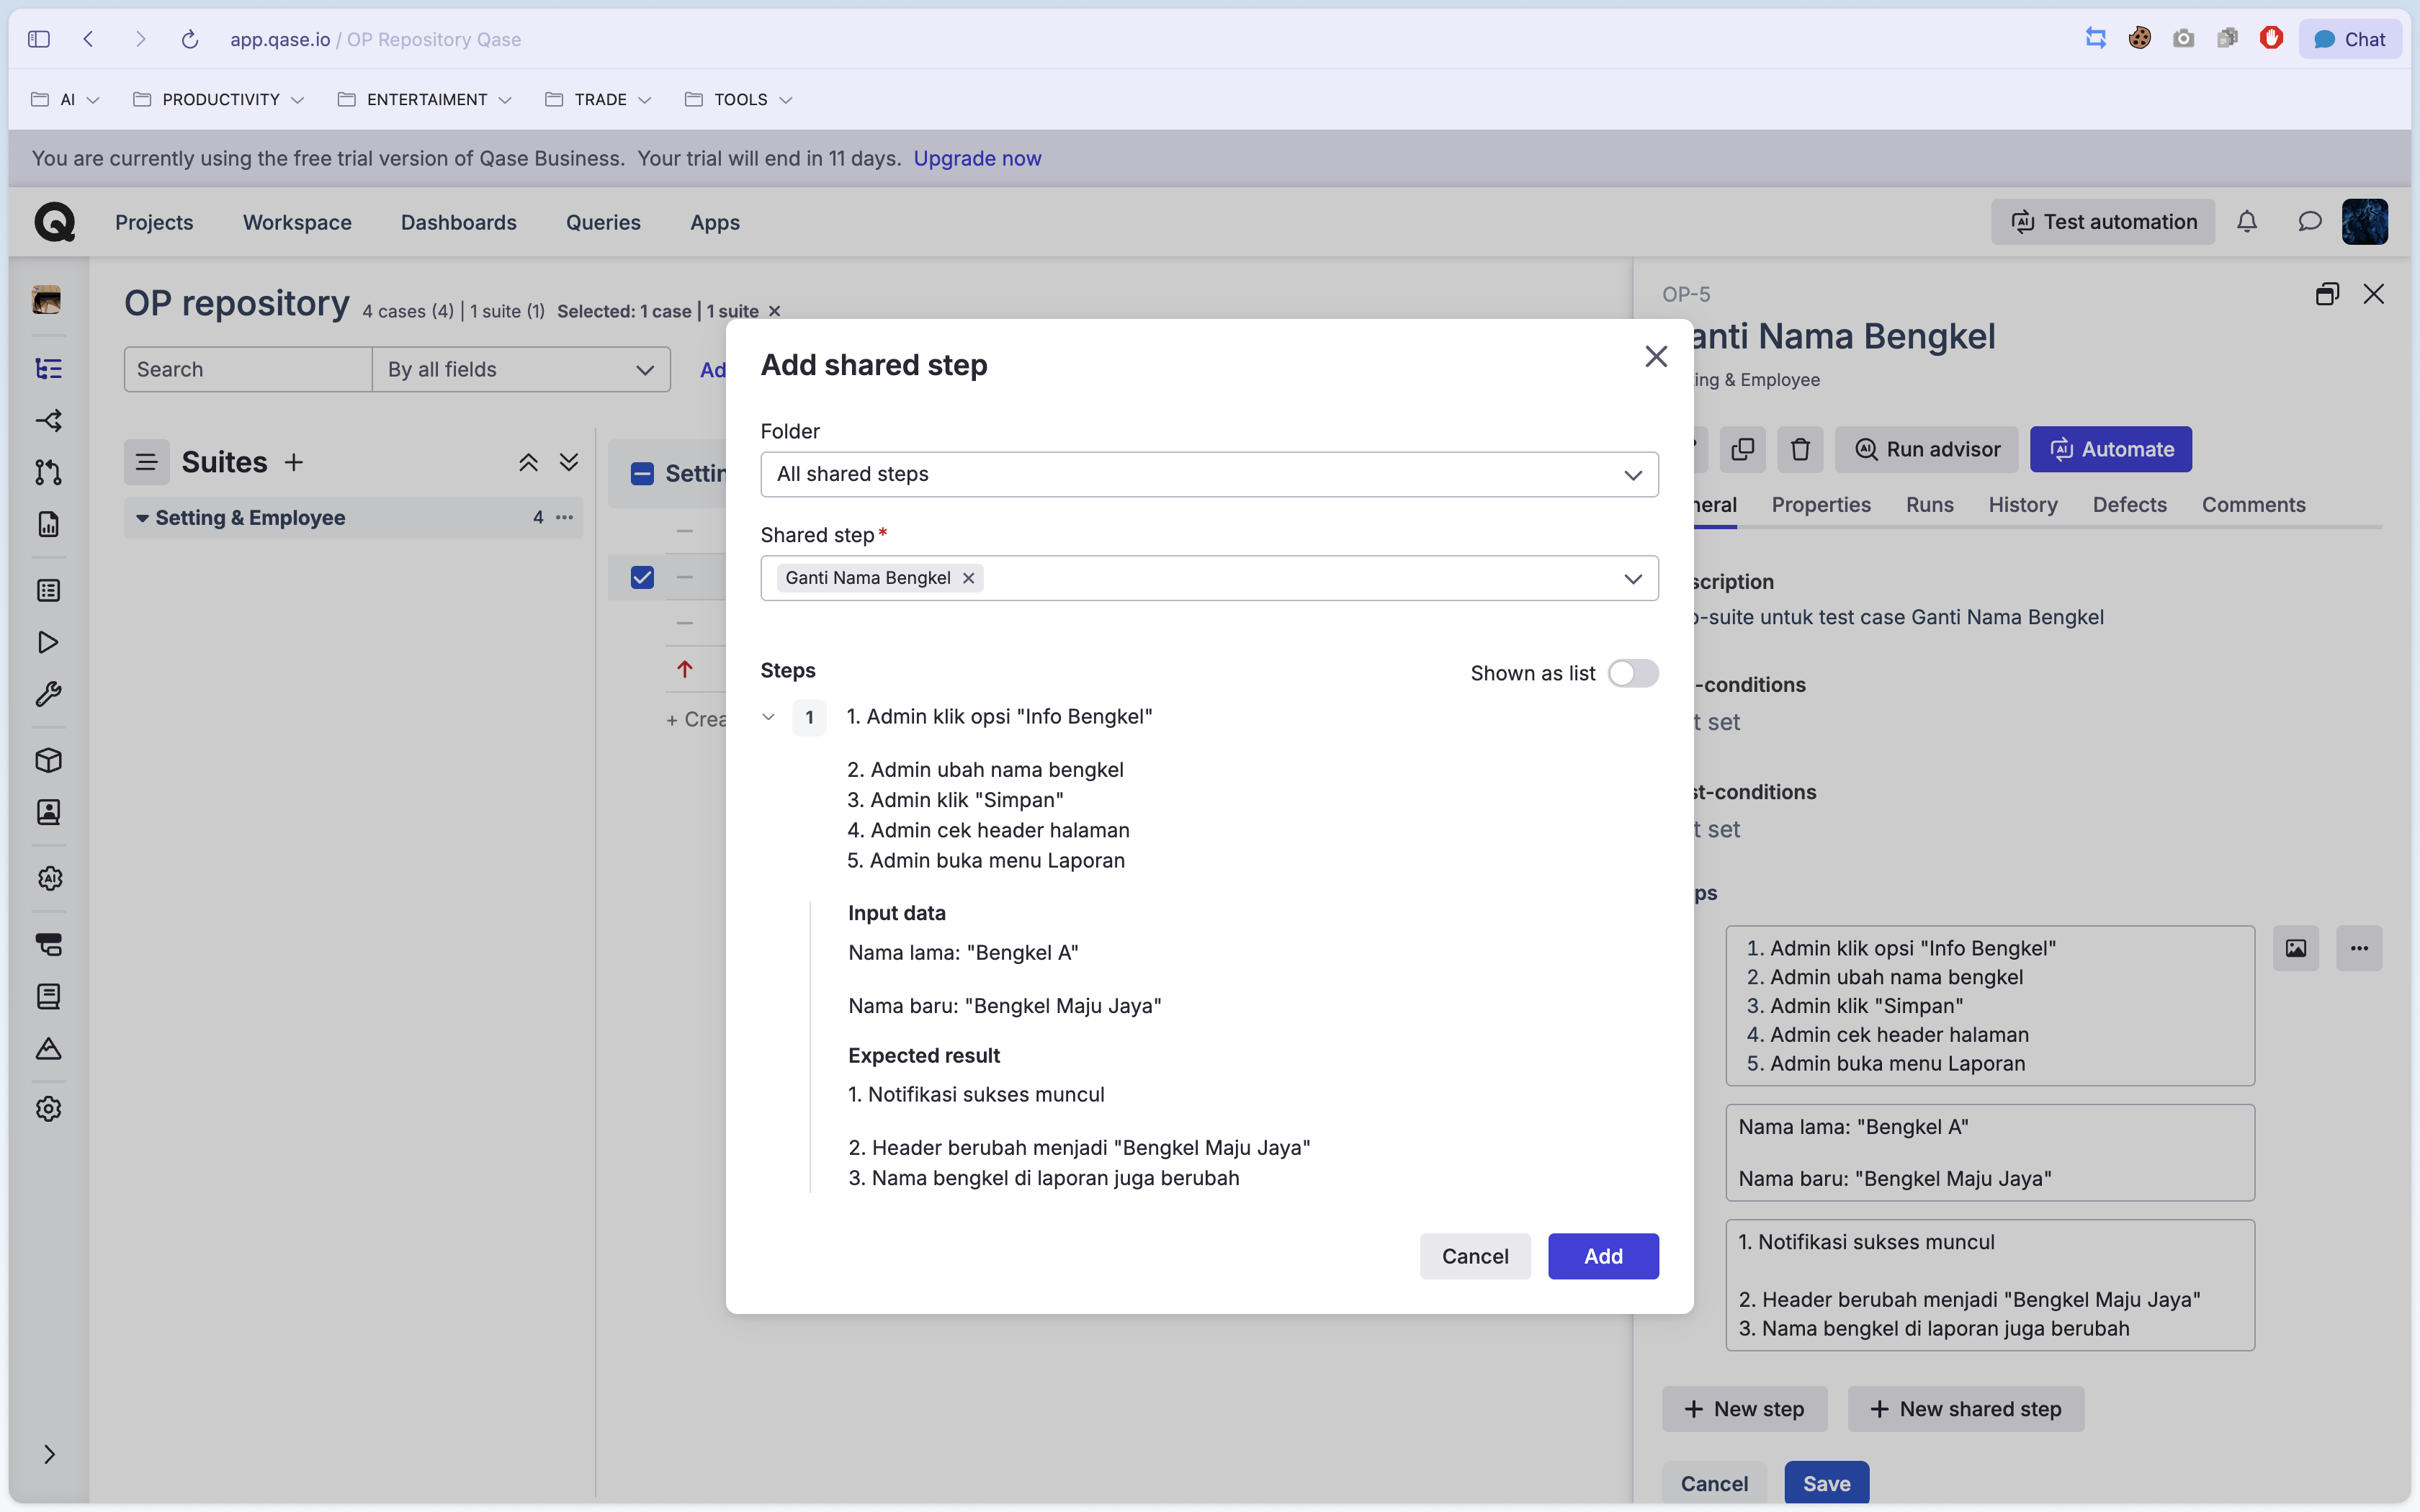
\includegraphics[width=\textwidth]{screenshot step/07-config shared step ke test case.png}
    \caption{Konfigurasi Shared Step ke Test Case}
\end{figure}

\subsection{Langkah 8: Membuat Environment}
Tahap ini bertujuan untuk mengatur variabel \textit{Environment} dimana aplikasi akan diuji, seperti Production atau Staging, agar konteks pengujian bisa dilacak dengan jelas.
\begin{figure}[H]
    \centering
    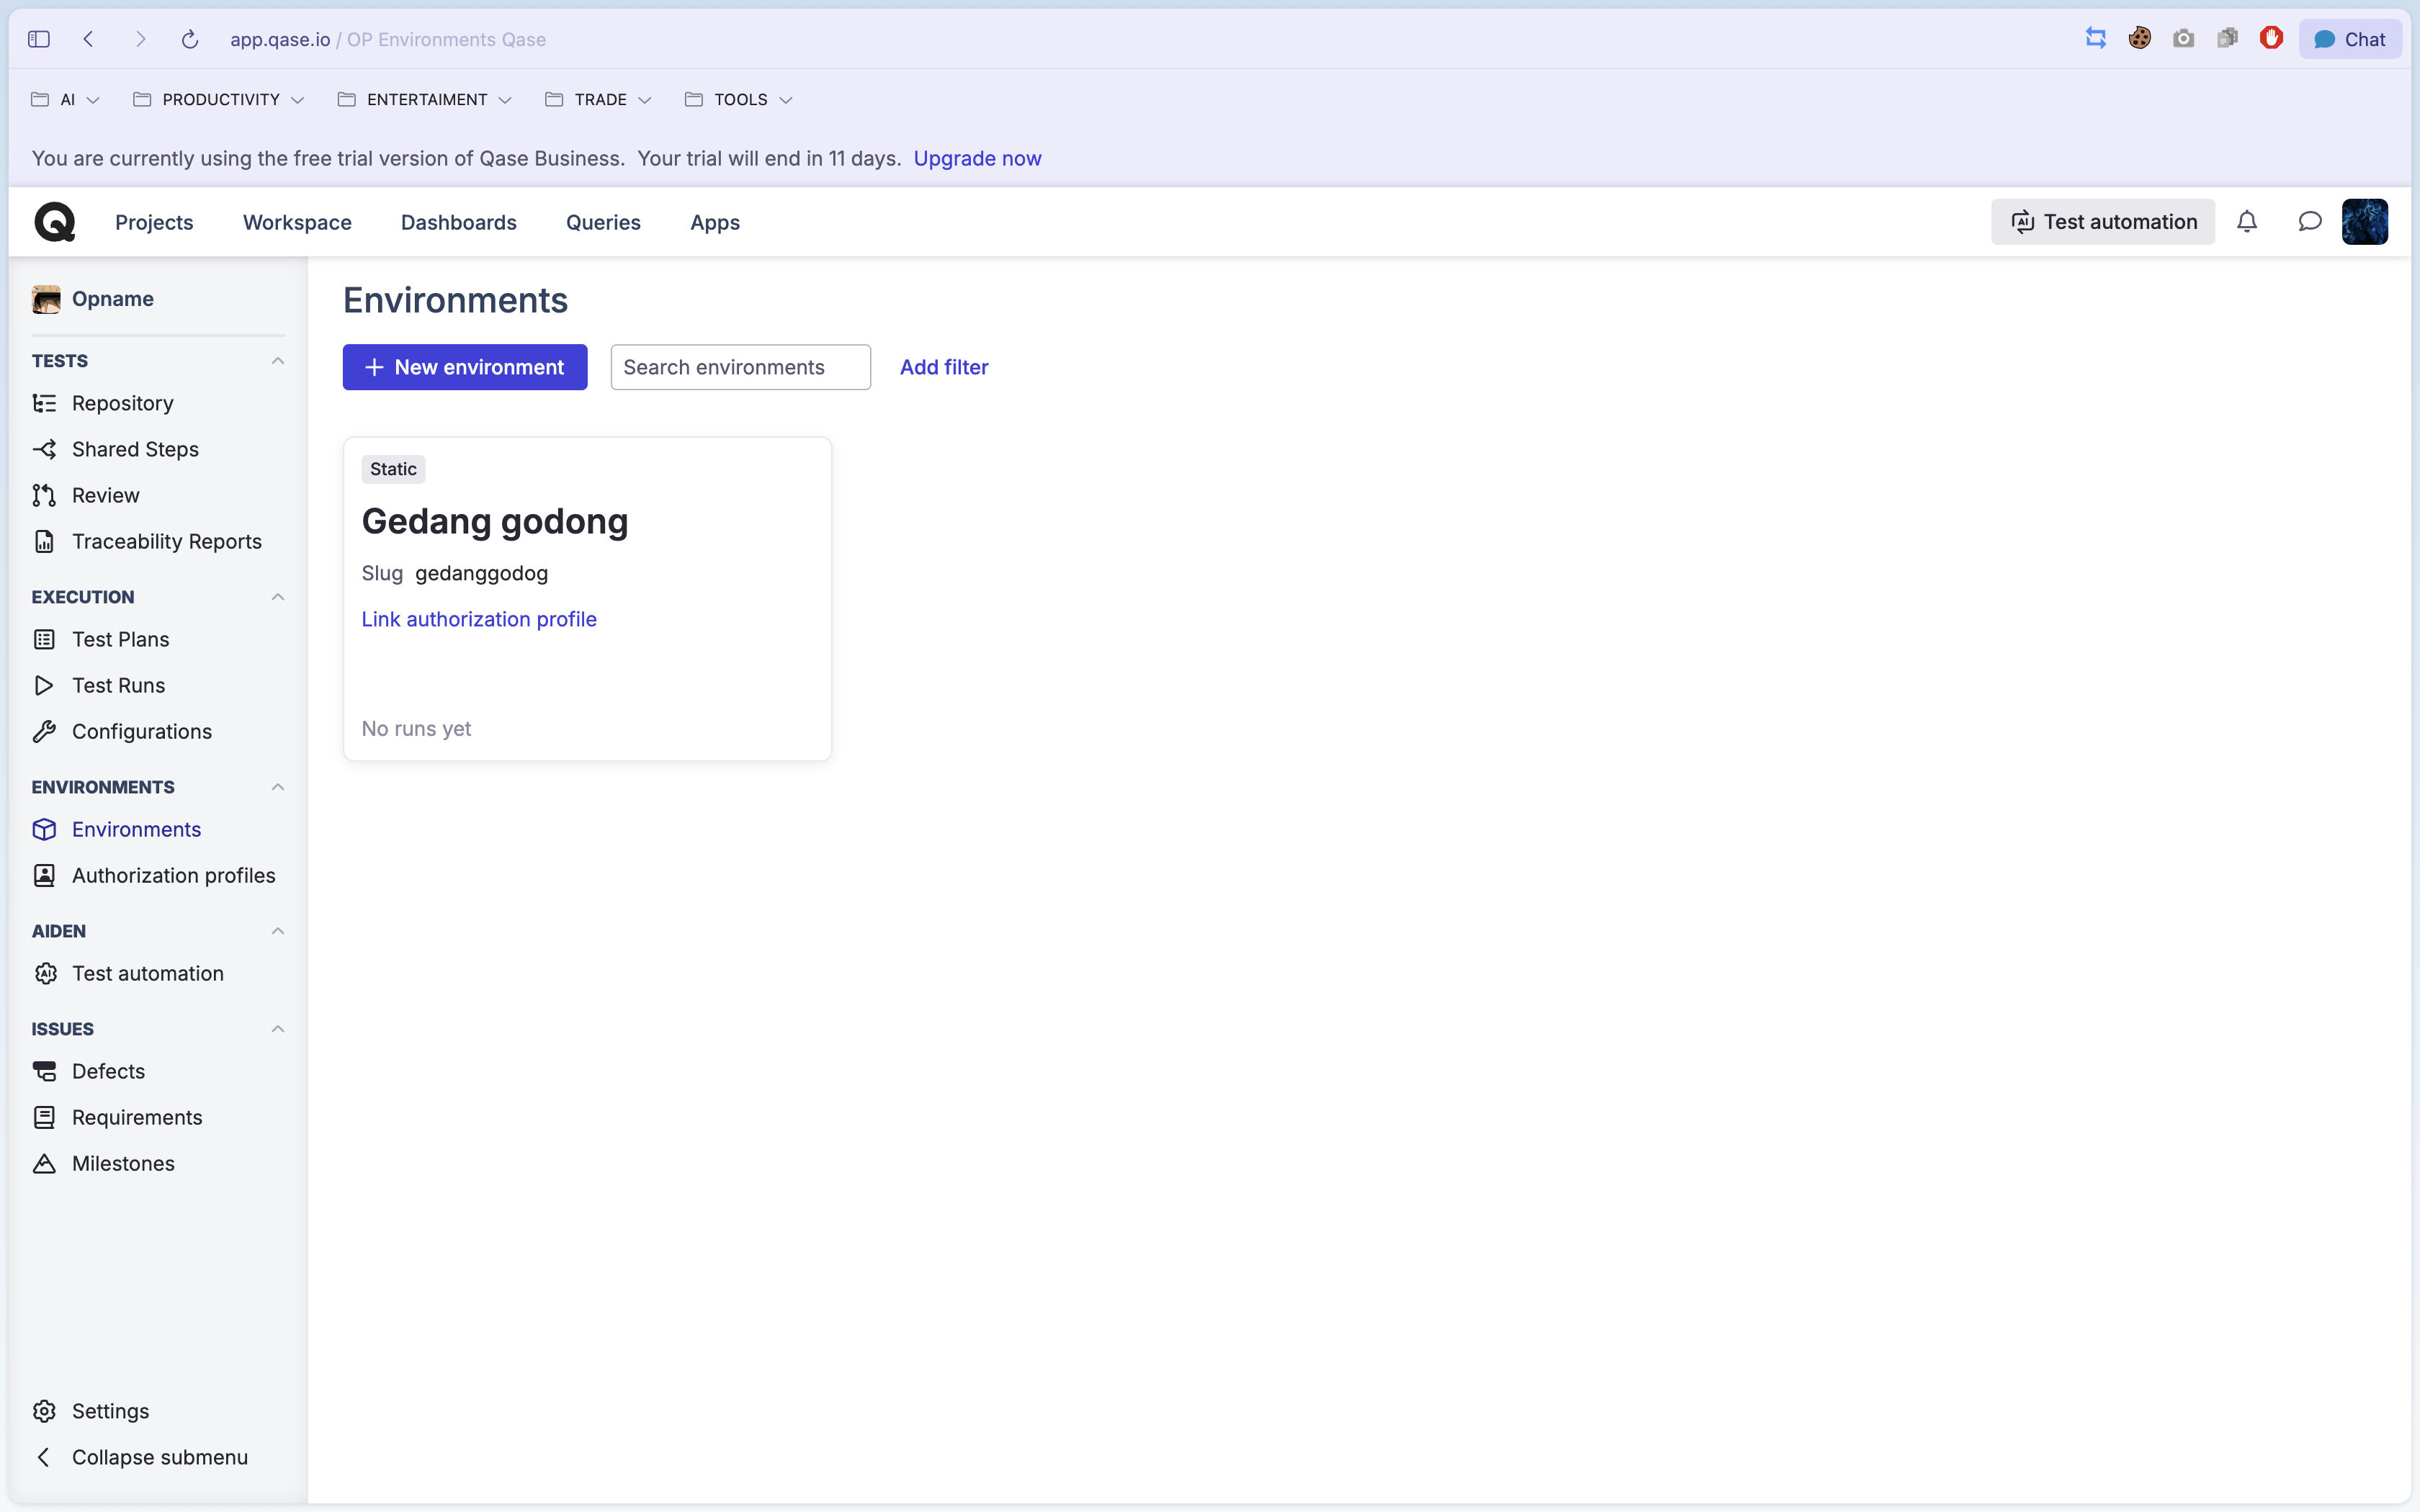
\includegraphics[width=\textwidth]{screenshot step/08-create env.png}
    \caption{Membuat Environment}
\end{figure}

\subsection{Langkah 9: Membuat Test Plan}
Kita merencanakan pelaksanaan dengan membuat \textit{Test Plan} yang mengelompokkan \textit{Test Suite} maupun \textit{Test Case} tertentu sebagai bagian dari lingkup perencanaan \textit{testing} di siklus tertentu.
\begin{figure}[H]
    \centering
    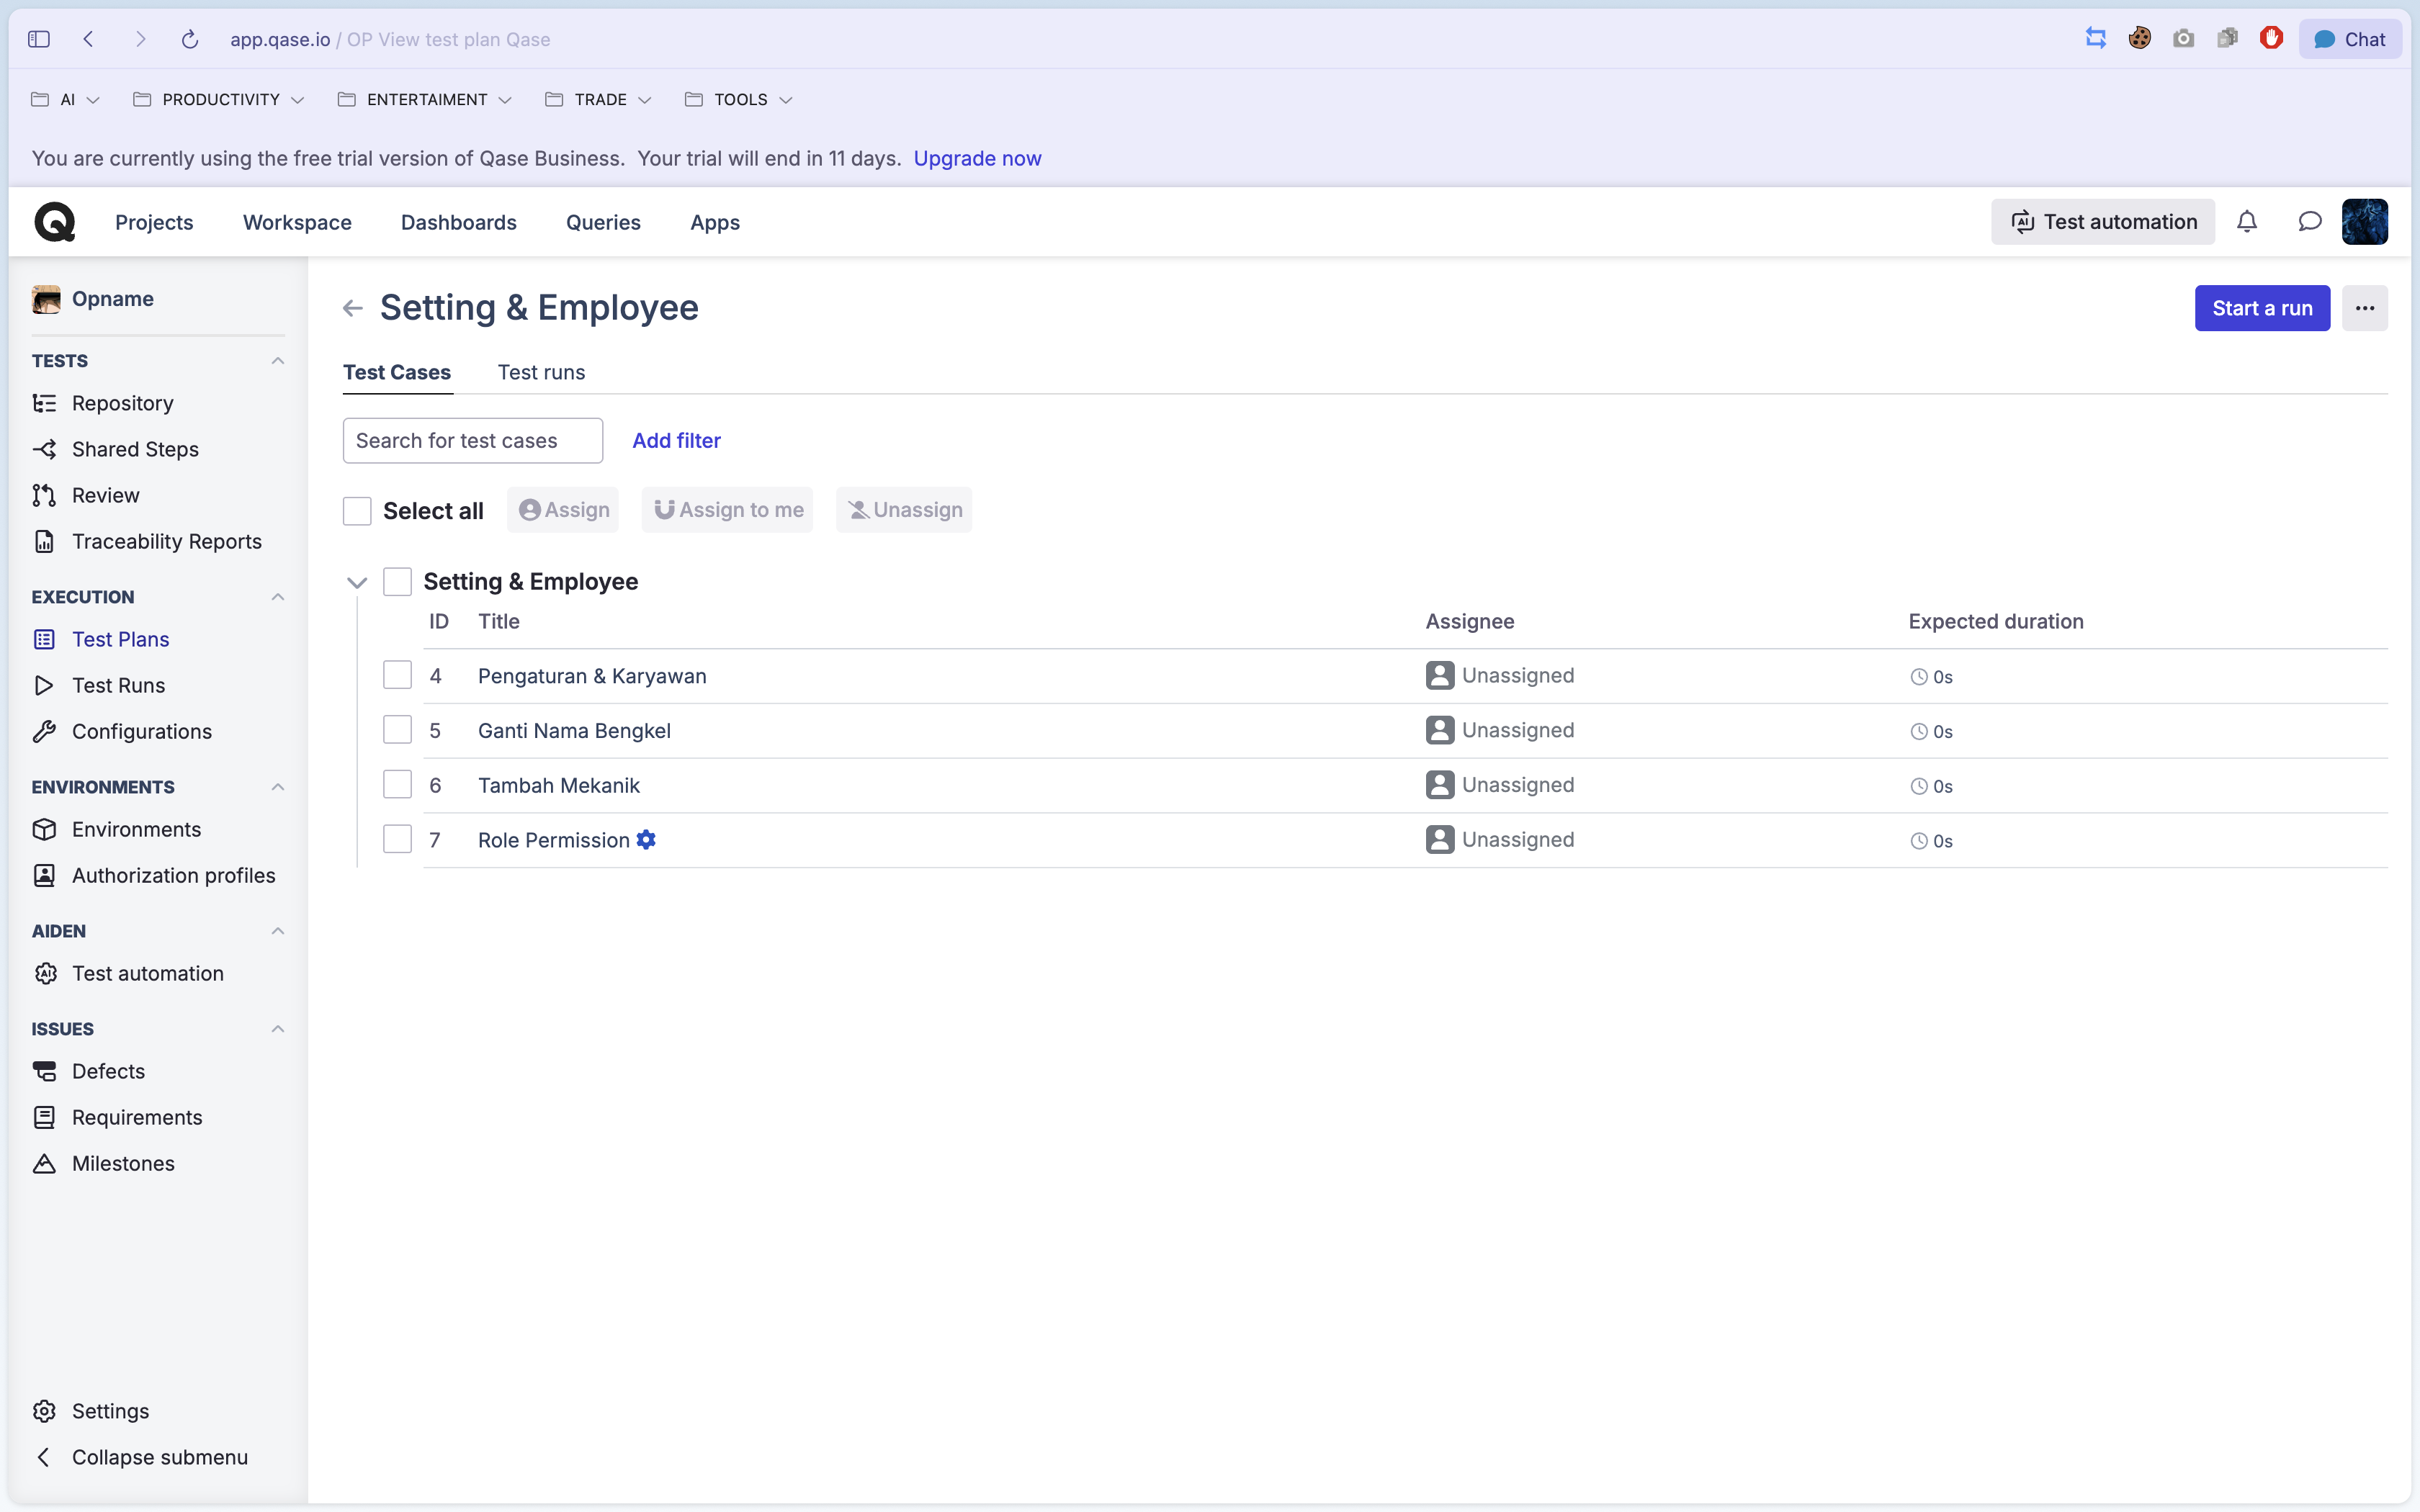
\includegraphics[width=\textwidth]{screenshot step/09-create testplan.png}
    \caption{Membuat Test Plan}
\end{figure}

\subsection{Langkah 10: Membuat Test Run Baru}
Lalu kita menginisisai eksekusi dengan membuat suatu \textit{Test Run} yang memuat \textit{Test Case} riil yang ditargetkan untuk segera dijalankan.
\begin{figure}[H]
    \centering
    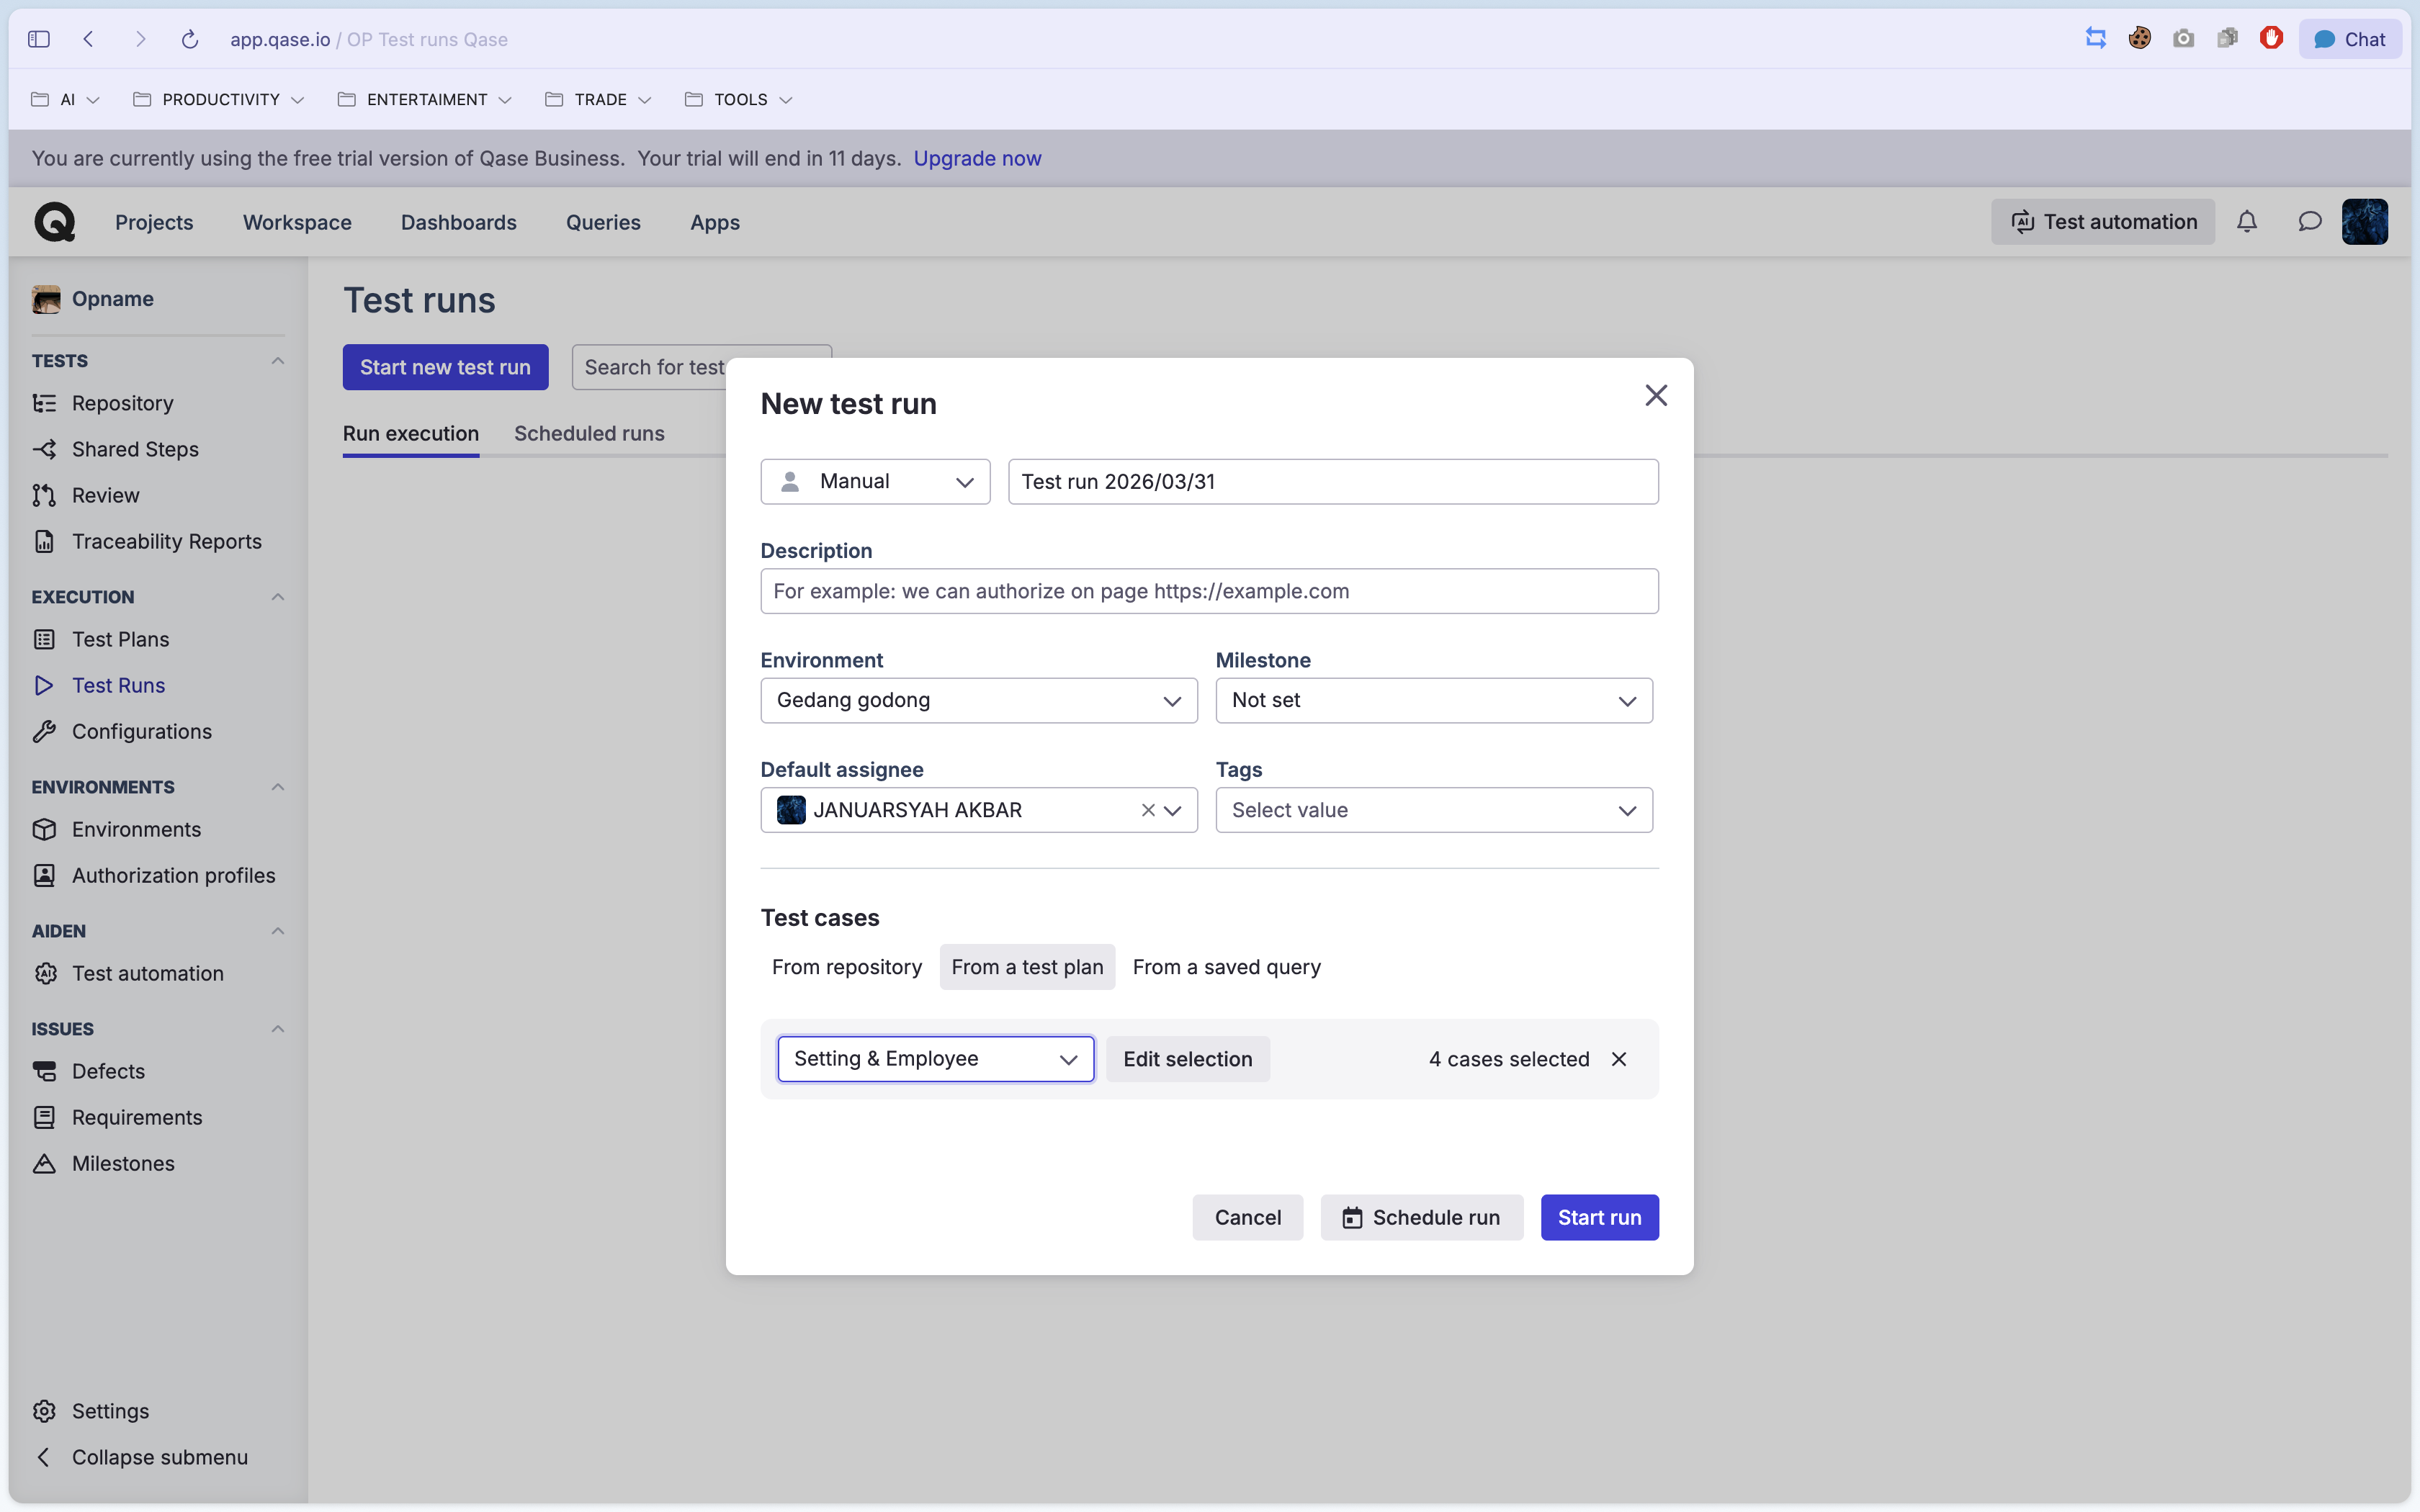
\includegraphics[width=\textwidth]{screenshot step/10-create new test run.png}
    \caption{Membuat Test Run Baru}
\end{figure}

\subsection{Langkah 11: Menjalankan Test Run}
Pada antarmuka pelaksanaan test ini, QA \textit{engineer} atau tester akan mereplikasi tahapan-tahapan yang ditentukan dan menandai hasilnya apakah berstatus \textit{Passed}, \textit{Failed}, atau \textit{Blocked}.
\begin{figure}[H]
    \centering
    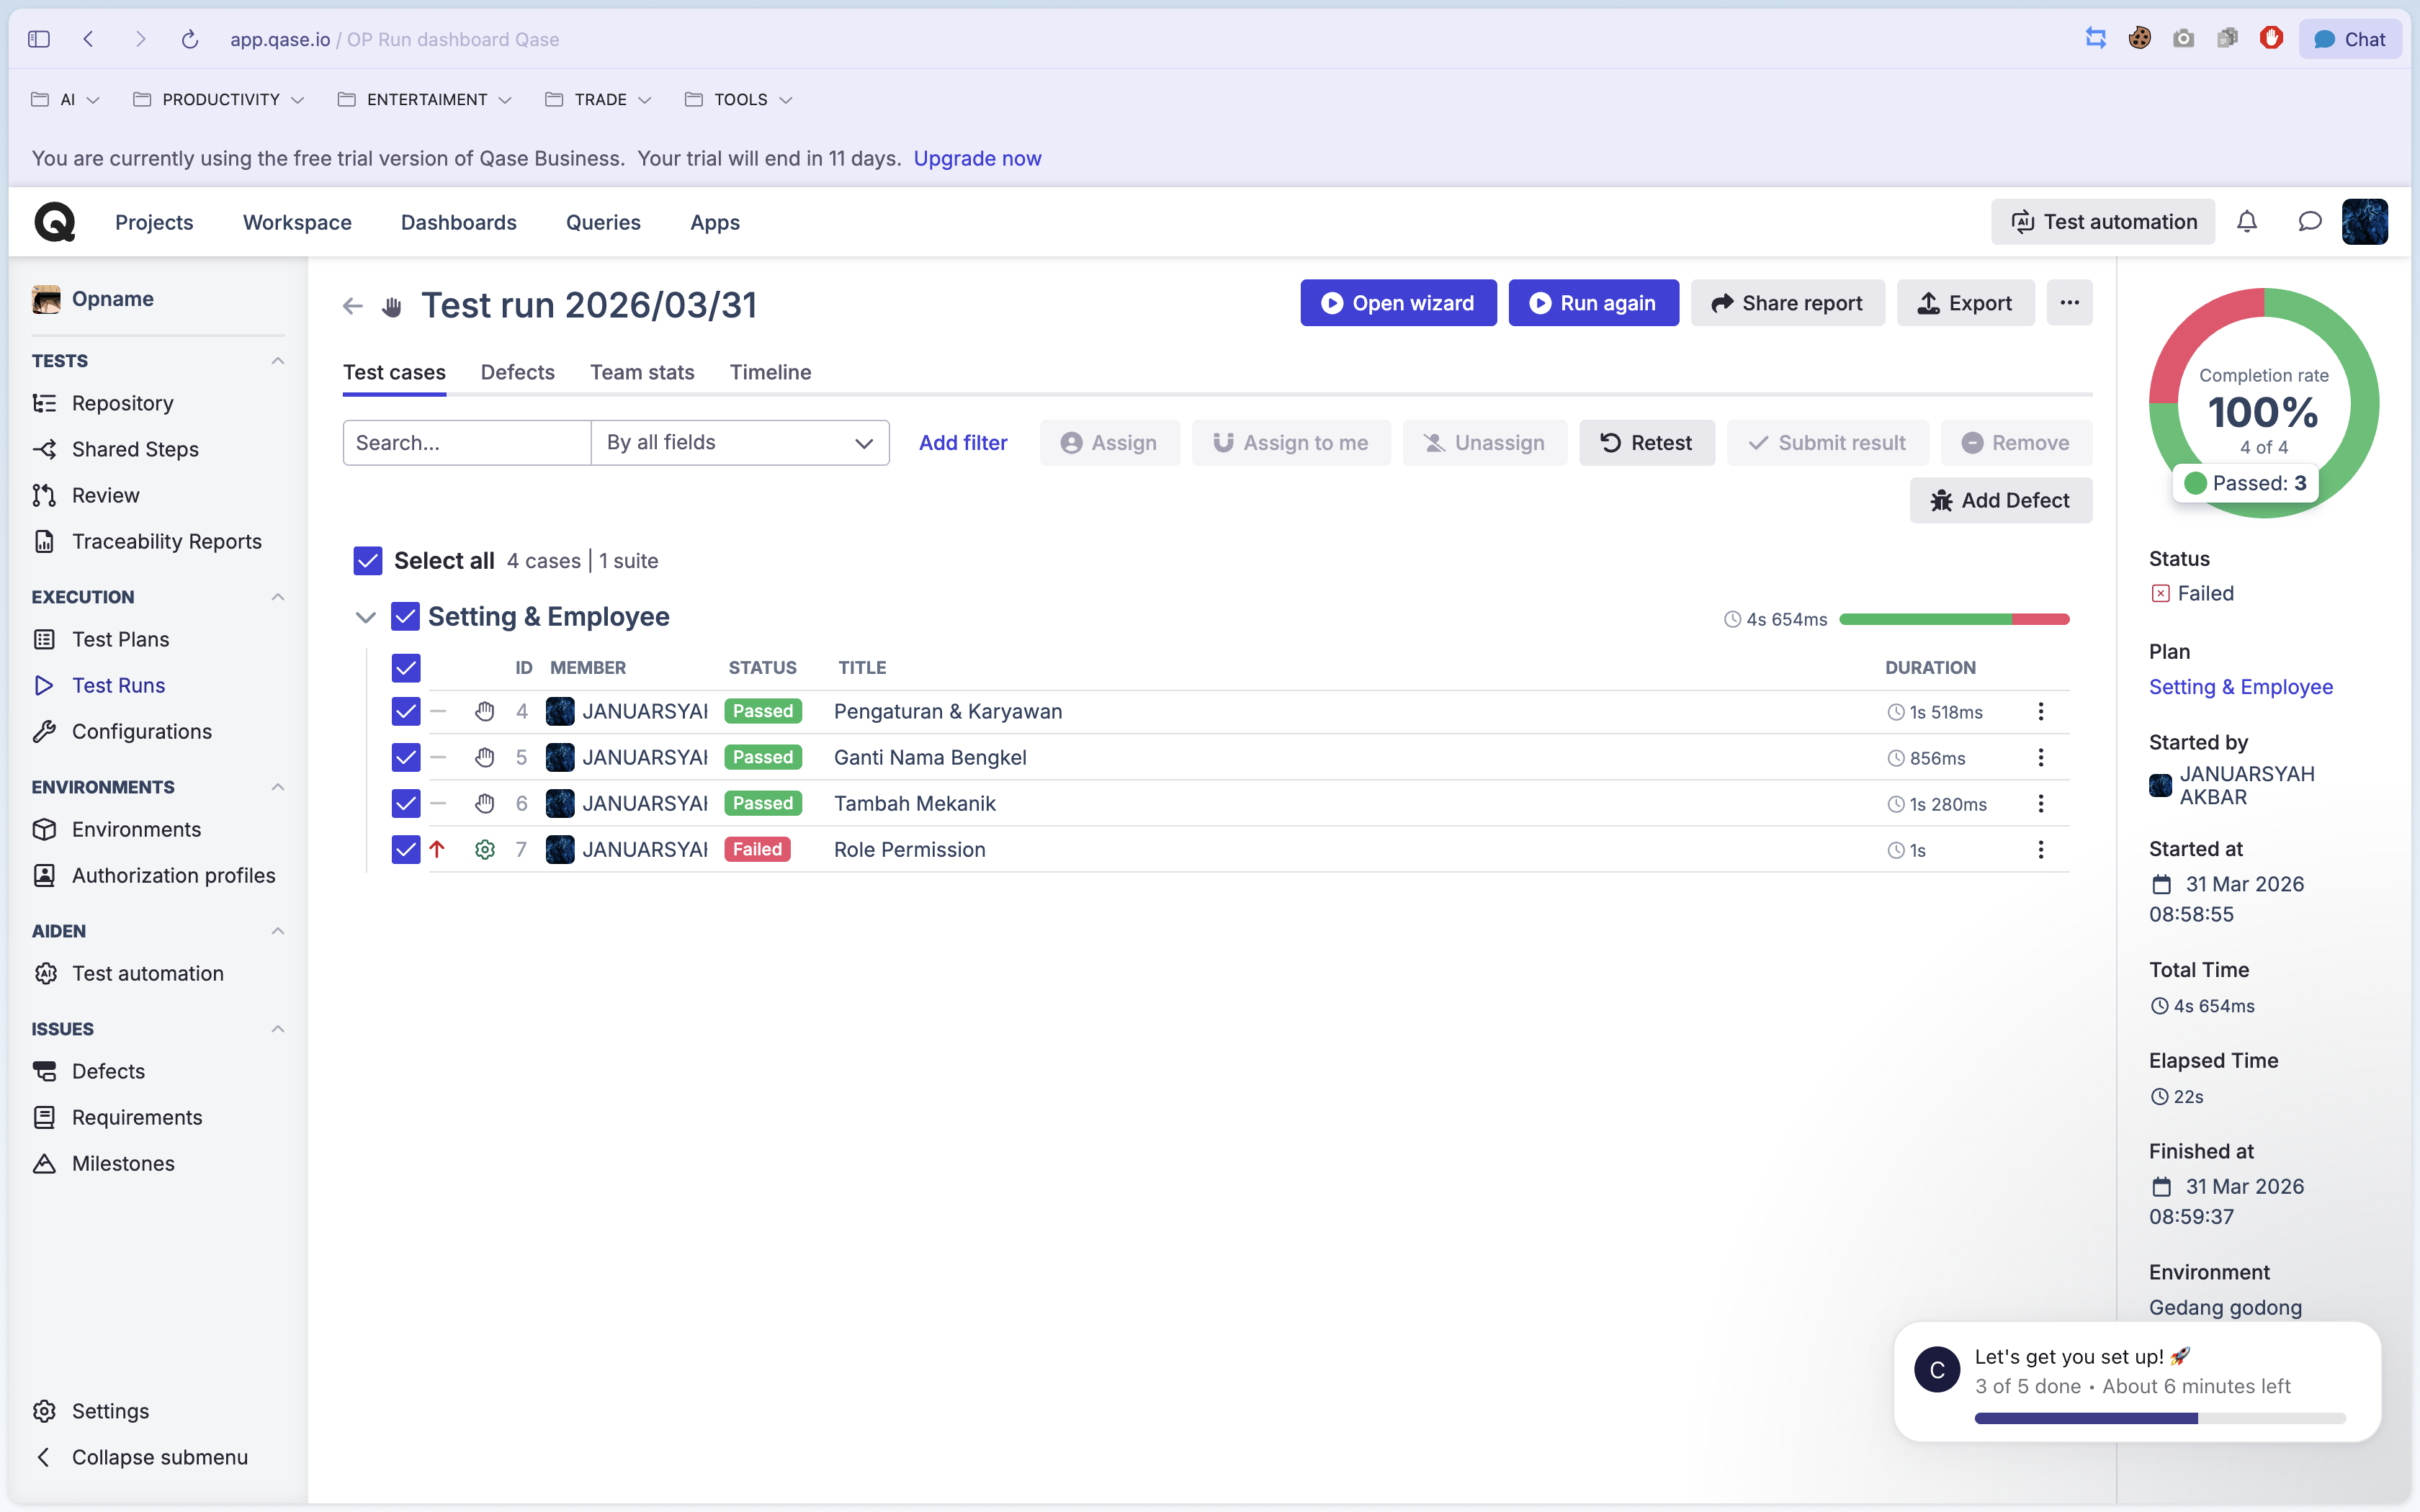
\includegraphics[width=\textwidth]{screenshot step/11-test run.png}
    \caption{Menjalankan Test Run}
\end{figure}

\subsection{Langkah 12: Membuat Bug Report}
Ketika ditemukan anomali atau fitur yang tidak menampilkan \textit{expected result}, maka langkah yang diambil ialah mendokumentasikan isunya pada sebuah tiket temuan masalah (\textit{Defect} atau \textit{Bug Report}).
\begin{figure}[H]
    \centering
    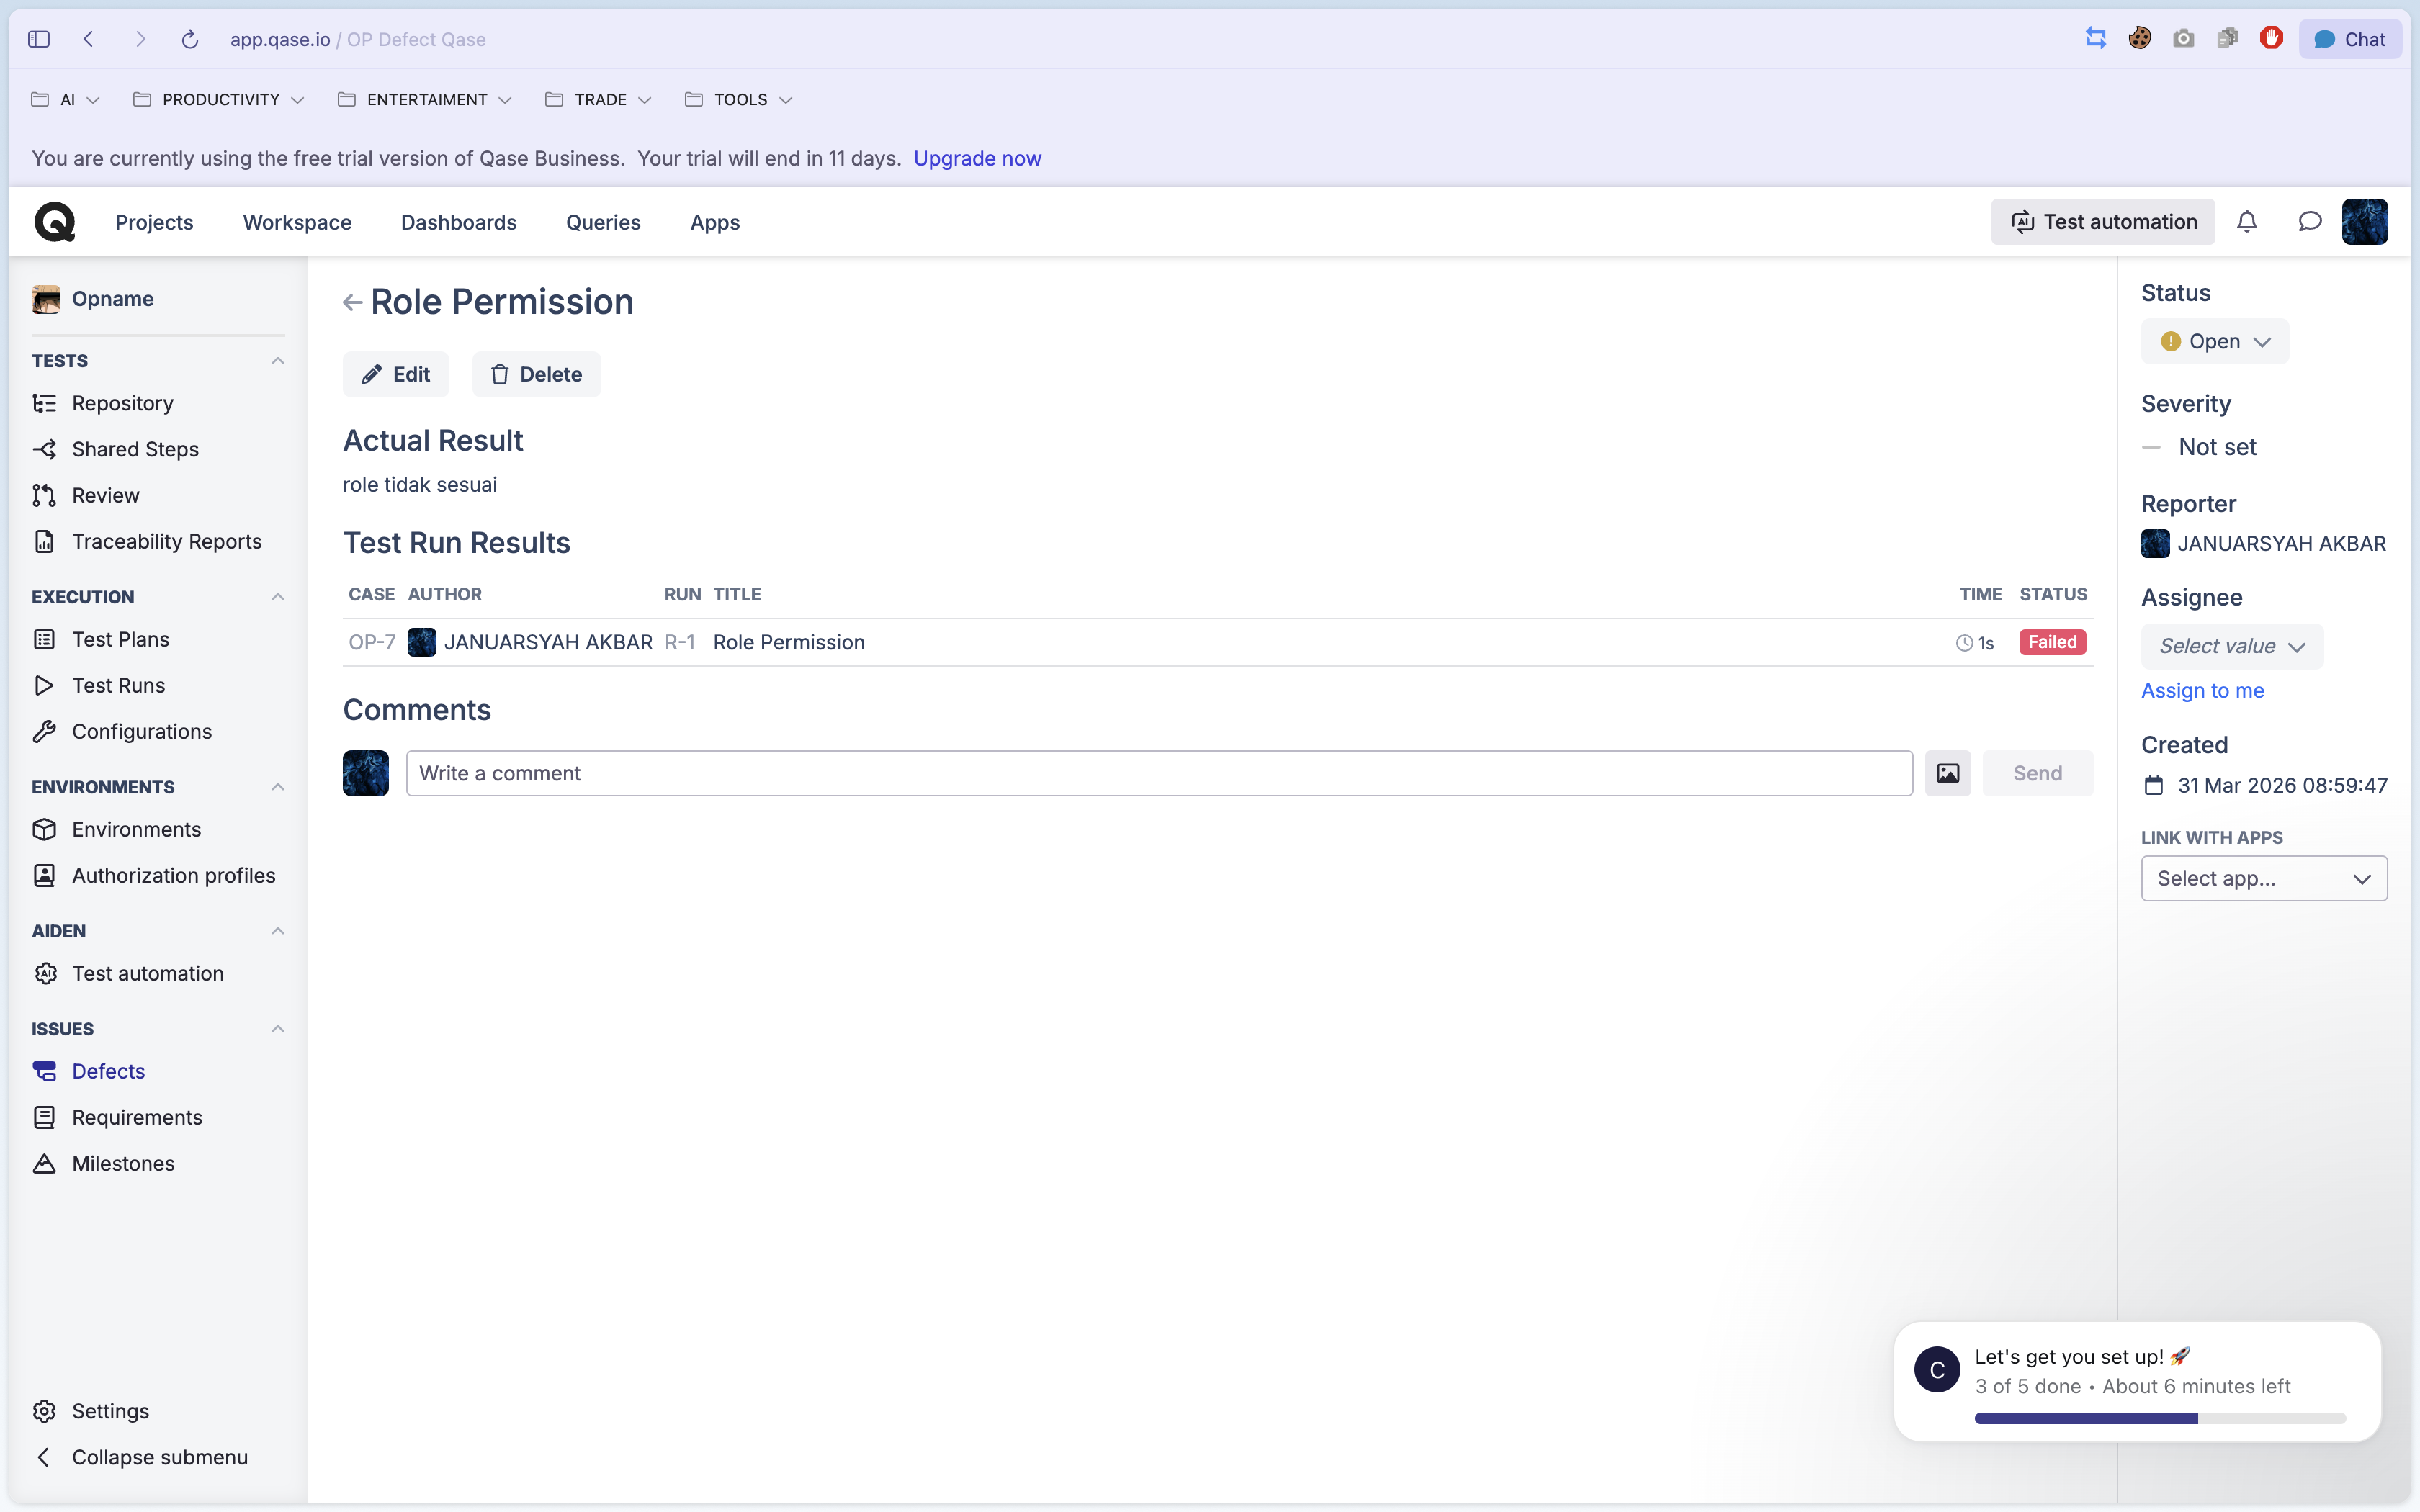
\includegraphics[width=\textwidth]{screenshot step/12-bug report.png}
    \caption{Membuat Bug Report}
\end{figure}

\subsection{Langkah 13: Melihat Daftar Defect}
Akhirnya, keseluruhan \textit{Defect} yang telah direkam selama tahapan \textit{Test Run} dapat disatukan dan dipantau kumpulannya pada halaman daftar Defect untuk ditindaklanjuti.
\begin{figure}[H]
    \centering
    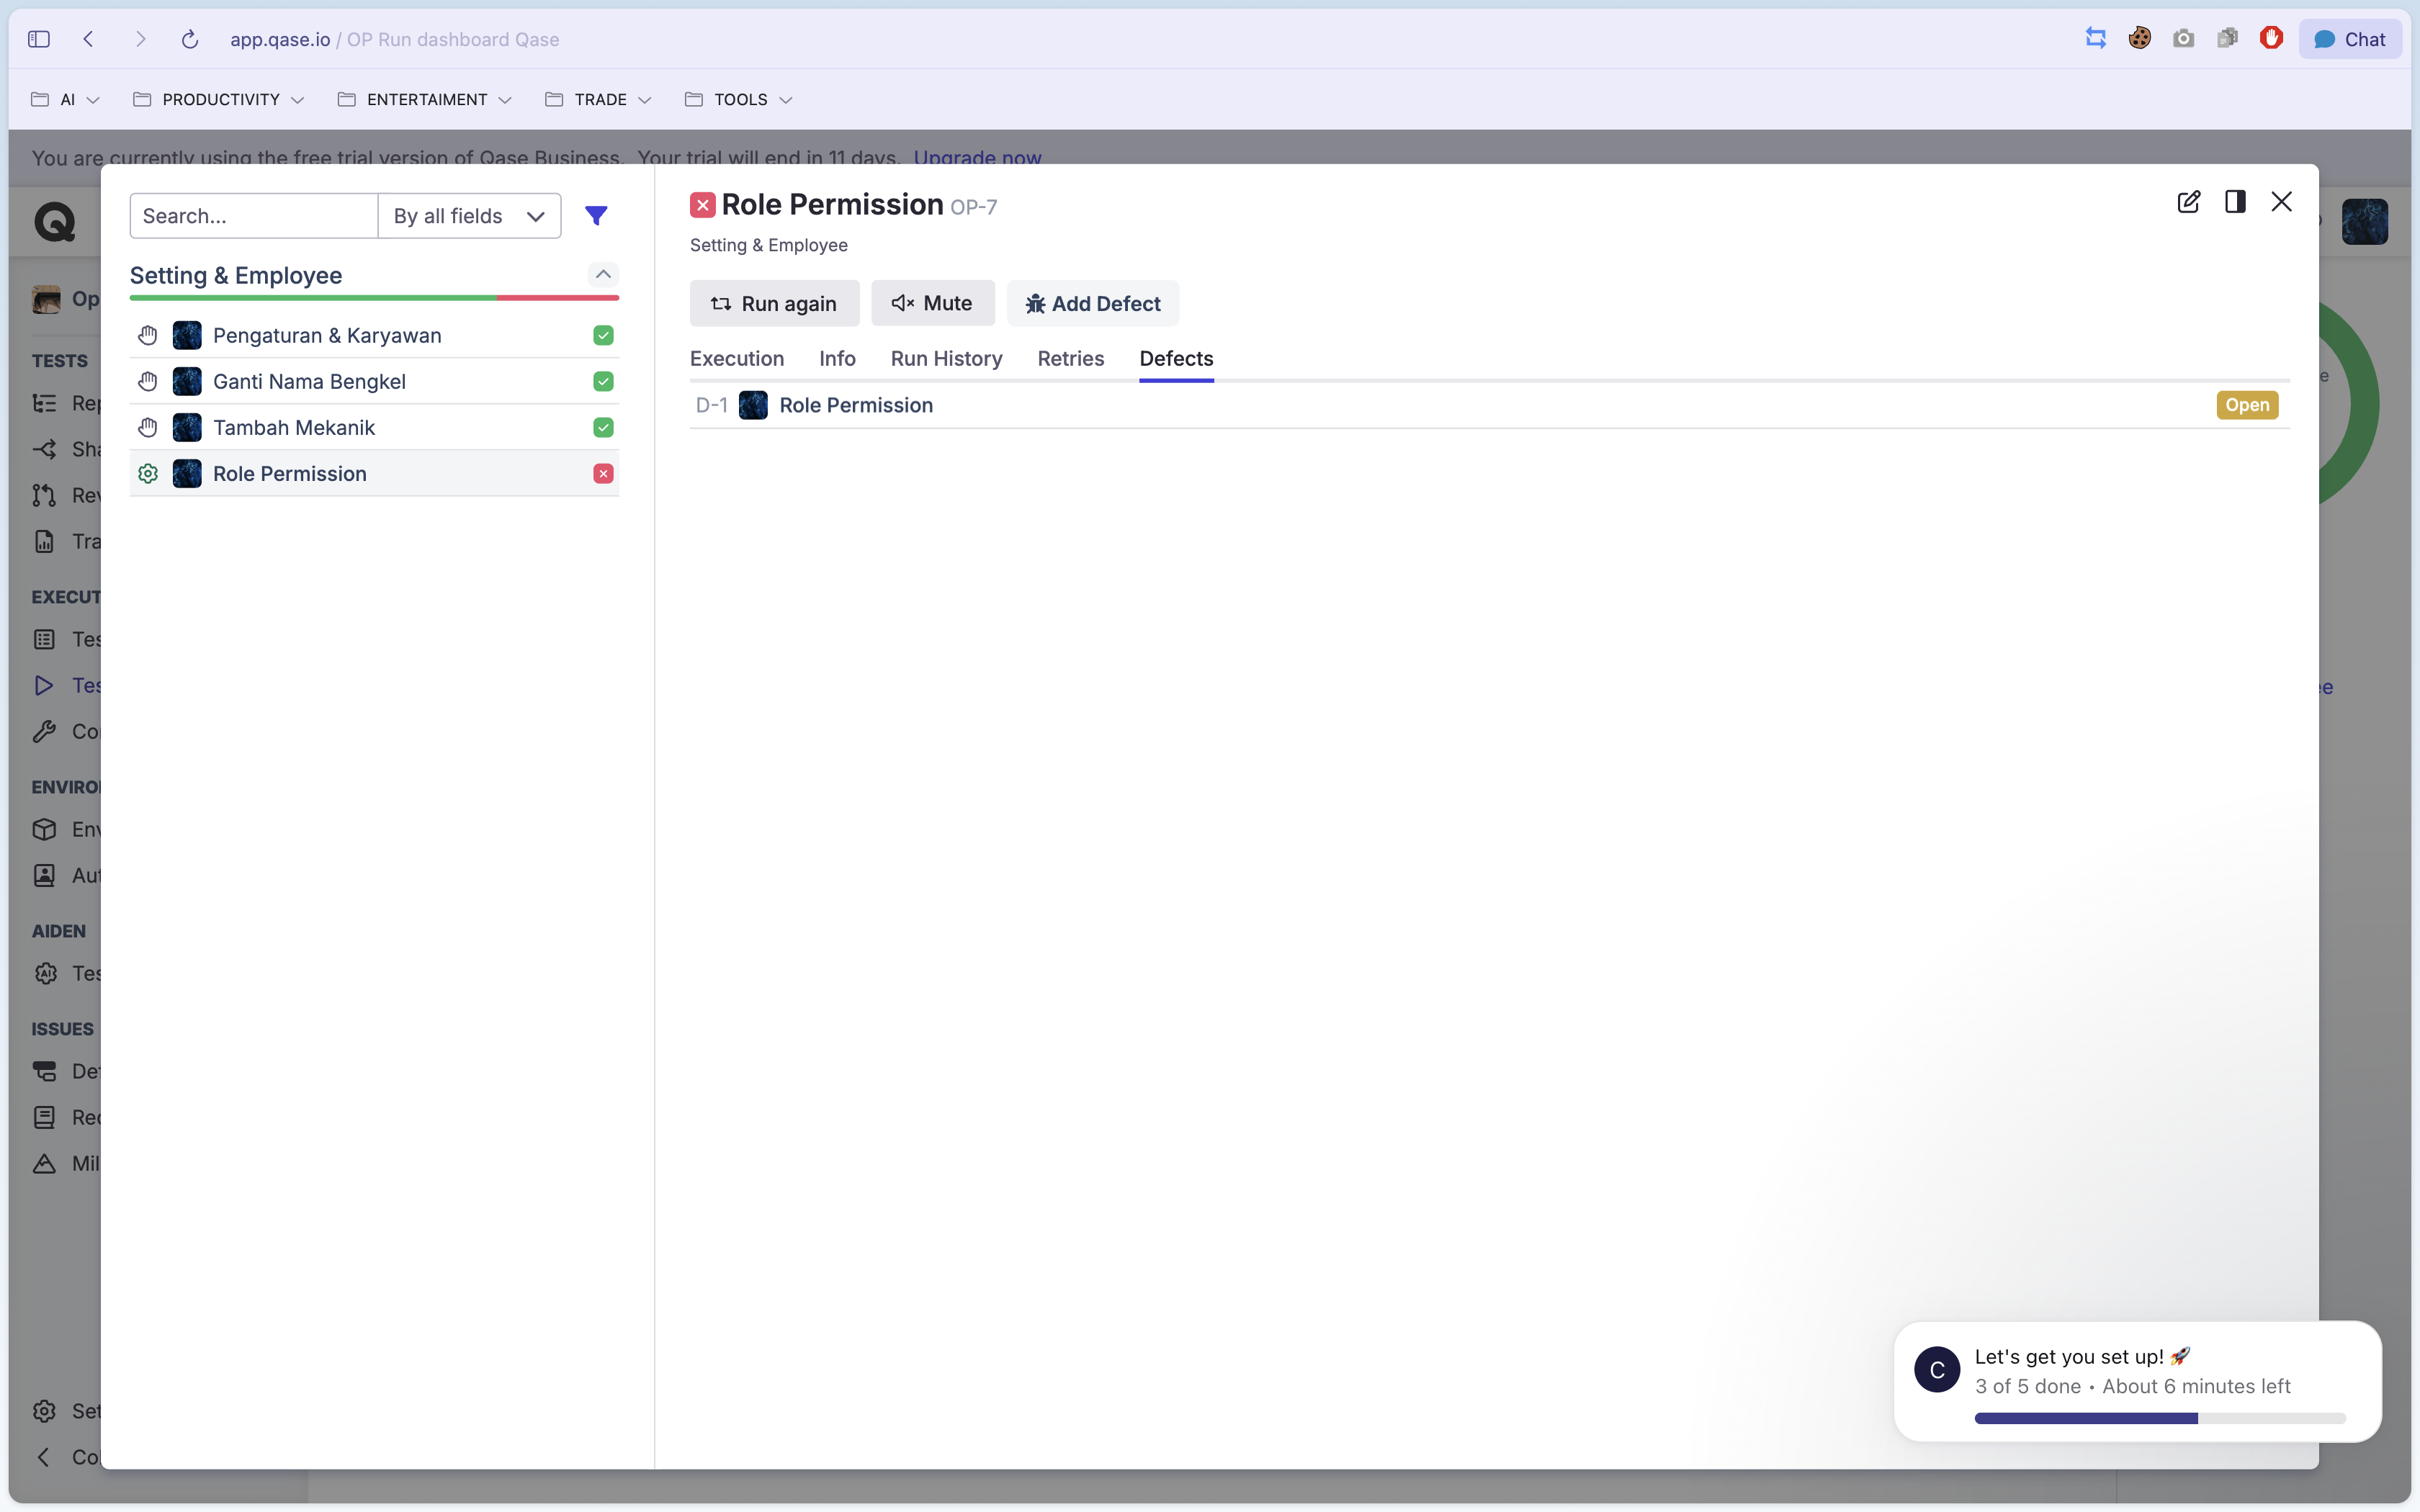
\includegraphics[width=\textwidth]{screenshot step/13-defact list.png}
    \caption{Melihat Daftar Defect}
\end{figure}

% \chapter{Resources}
% %======================================================================

% \begin{center}
%     \url{https://github.com/januarsyah901/PPPL/tree/9d622d374dcf5c9e04c560607ba4e59049f3681a/Pertemuan%204}
% \end{center}

\clearpage

%======================================================================
\chapter{Kesimpulan}
%======================================================================

Berdasarkan praktikum yang telah dilakukan, dapat disimpulkan bahwa penggunaan \textit{Test Management Tool} sangat mempermudah pendokumentasian dan pelaksanaan pengujian perangkat lunak secara lebih terstruktur. Seluruh proses mulai dari pembuatan \textit{Project}, \textit{Test Suite}, penyusunan \textit{Test Case}, \textit{Test Plan}, hingga pelaksanaan \textit{Test Run} dapat dikelola secara terpusat dan saling terintegrasi. 

Selain itu, pendokumentasian tahapan pengujian menjadi lebih efisien dengan adanya fitur \textit{Shared Step}. Apabila terdapat anomali atau kegagalan tes selama pelaksanaan, temuan tersebut dapat langsung dicatat menjadi \textit{Defect} atau \textit{Bug Report} yang tersistematis pada satu \textit{environment} yang sama. Hal ini akan sangat mempermudah tim \textit{Developer} dan QA dalam melacak (\textit{tracking}), menganalisis, serta meresolusi permasalahan dalam sistem aplikasi perangkat lunak secara lebih praktis.

% \clearpage
% \addcontentsline{toc}{chapter}{Daftar Pustaka}
% \renewcommand{\bibname}{Daftar Pustaka}

% \begin{thebibliography}{99}
%     \bibitem{mockito} Mockito Project, ``Mockito --- tasty mocking framework for unit tests in Java''. [Online]. Tersedia: \url{https://site.mockito.org/}.
%     \bibitem{junit5} JUnit Team, ``JUnit 5 User Guide''. [Online]. Tersedia: \url{https://junit.org/junit5/docs/current/user-guide/}.
%     \bibitem{fowler-mocks} Martin Fowler, ``Mocks Aren't Stubs'', 2007. [Online]. Tersedia: \url{https://martinfowler.com/articles/mocksArentStubs.html}.
% \end{thebibliography}

\end{document}
